% AER-Article.tex for AEA last revised 22 June 2011
\documentclass[AER]{AEA}

% The mathtime package uses a Times font instead of Computer Modern.
% Uncomment the line below if you wish to use the mathtime package:
%\usepackage[cmbold]{mathtime}
% Note that miktex, by default, configures the mathtime package to use commercial fonts
% which you may not have. If you would like to use mathtime but you are seeing error
% messages about missing fonts (mtex.pfb, mtsy.pfb, or rmtmi.pfb) then please see
% the technical support document at http://www.aeaweb.org/templates/technical_support.pdf
% for instructions on fixing this problem.

% Note: you may use either harvard or natbib (but not both) to provide a wider
% variety of citation commands than latex supports natively. See below.

% Uncomment the next line to use the natbib package with bibtex 
\usepackage{natbib}

% Uncomment the next line to use the harvard package with bibtex
%\usepackage[abbr]{harvard}

% This command determines the leading (vertical space between lines) in draft mode
% with 1.5 corresponding to "double" spacing.

\usepackage[table,xcdraw]{xcolor}
\usepackage{caption}
\usepackage{subcaption}
\usepackage{graphicx}

\draftSpacing{1.5}

\begin{document}

\title{Social norms, incentives, and prosocial behavior}
\shortTitle{Social norms, incentives, and prosocial behavior}
\author{Caroline Graf, Bianca Suanet, Pamala Wiepking and\\ Eva-Maria Merz\thanks{We are grateful to Wim de Kort and all blood donation experts from across Europe who shared their knowledge about incentives for donors in their countries with us. Moreover, we thank Joris Schroeder for valuable discussions about this project. Correspondence concerning this working paper should be addressed to Caroline Graf (c.graf@vu.nl) or Eva-Maria Merz (e.m.merz@vu.nl).}}
\date{\today}
\pubMonth{September}
\pubYear{2020}
\pubVolume{}
\pubIssue{}
\JEL{}


\begin{abstract}
Incentives have surprisingly inconsistent effects when it comes to encouraging people to behave prosocially. That is, the effects of incentives vary across incentive types, private versus public settings and across countries. Previous theoretical accounts have aimed at explaining these empirical phenomena by postulating an additive effect of intrinsic motivation, extrinsic motivation, reputational motivation, and costs. We build on these theories, but call into question whether reputational motivation can be derived a priori, for instance by assuming an immutable cost to being perceived as extrinsically motivated. Instead, we argue that reputational concerns are governed by social norms, that is how acceptable certain actions are viewed by members of society. We go on to test our model comparatively on the real-world prosocial behavior of blood donation. We find that financial incentives have a direct negative effect on prosociality, and that social norms regarding financial incentives were rather negative, with the majority of the population in all countries considering them unacceptable. However, those respondents in countries with more positive social norms were more likely to have donated blood. On the other hand, social norms regarding non-financial incentives were substantially more positive compared to those regarding financial incentives. Crucially, the more positive the country-level social norms were, the more likely were individuals residing in these countries to have donated, when non-financial incentives were offered in this country. The results indicate that social norms regarding incentives play an important role in determining the effect of incentives on prosocial behavior.

\textbf{Keywords}: {\normalfont prosocial behavior, incentives, social norms, blood donation, reputation, intrinsic motivation, extrinsic motivation}
\end{abstract}


\maketitle

Humans are remarkable in the extent to which they engage in prosocial behavior -- and many communities want to encourage their members to help each other and contribute to public goods. According to classical economic theory, an obvious means to do this is by offering incentives \citep{mill_principles_1882}. For instance, tax breaks can be implemented to incentivize charity donations or blood donors can be remunerated to ensure a steady blood supply. However, incentives sometimes backfire, and can actually have detrimental effects on prosocial behavior \citep{deci_effects_1971, gneezy_pay_2000, gneezy_fine_2000}. Under which circumstances do incentives encourage prosocial behavior?

\paragraph{Inconsistent effects of incentives on prosocial behavior}

Empirical evidence examining the impact of incentives, that is as \textit{extrinsic rewards}\footnote{We follow \cite{chell_systematic_2018} in defining an incentive as an “extrinsically motivated reward, which can be monetary or nonmonetary and is used to motivate an action” (p.245). Extrinsic rewards are the positive \textit{external} outcomes that are associated with a given behavior, such as financial rewards, gifts or medals; this is opposed to \textit{intrinsic rewards} which are the positive \textit{internal} outcomes of a behavior, such as the simple pleasure in performing the behavior.}, on prosocial behavior has been inconsistent. On the one hand, it has been demonstrated that incentives sometimes encourage prosocial behavior \cite[e.g., tax breaks increase charitable giving; ][]{duquette_tax_2016}. A positive effect of incentives has also been found specifically for blood donation: For instance, \cite{goette_blood_2020} showed that lottery tickets increase donations, especially among less motivated donors. Similarly, \cite{lacetera_economic_2013} summarize evidence from observational and field studies, where 18 of the 19 offered incentive items (e.g., material rewards, lottery tickets, gift cards) increased blood donations, and this effect was stronger the higher the monetary value of the item. On the other hand, incentives can also have \textit{detrimental} effects on the amount of prosocial behavior exhibited. For instance, high school students going door-to-door to collect donations have been shown to gather \textit{less} donations when being paid proportional to the charitable donations they collected than if they were not paid \citep{gneezy_pay_2000}. Indeed, reviews both in economics \citep{gneezy_when_2011} and in the blood donation literature \citep{chell_systematic_2018} conclude that the effectiveness of incentives to encourage prosocial behavior is strongly \textit{context-dependent}. 

However, a myriad of factors is subsumed within this large bin of “context dependency”. One type of context effects are \textit{methodological} context effects. For example, it has been shown that substantial variation exists across studies using different data acquisition methods: Surveys tend to find that \textit{attitudes} oppose incentives (i.e., people tend to report in surveys that they are not attracted by incentives), whereas experiments and observational studies more often find positive effects of incentives on actual \textit{behavior} \cite[i.e., the amount of prosocial behavior tends to be positively affected by incentives; ][]{chell_systematic_2018}. Another set of context effects refers to the \textit{type and value} of the incentive provided (e.g., blood donation behavior was increased more when incentives with higher value were provided \citep{lacetera_economic_2013} \footnote{Interestingly, the opposite effect for type of incentives was found for \textit{attitudes}: Survey respondents were shown to mostly have negative attitudes toward receiving financial rewards for blood donation, whereas attitudes toward receiving non-financial incentives such as small gifts and medical tests tended to be more positive \citep{lacetera_economic_2013}.}. Lastly, \textit{societal} context which varies across studies conducted in different countries and operating contexts has been shown to impact the effect of incentives on prosocial behavior \citep{chell_systematic_2018}. In the current paper we focus specifically on the effects of \textit{societal context}\footnote{With societal context we refer specifically to the prevailing social norms toward incentives in a society, as well as the country-level policies regarding incentives for donors.} as well as \textit{incentive type} on prosocial behavior, taking blood donation as a real-world example for prosocial behavior. 

\paragraph{Deterioration of \textit{intrinsic} motivation by extrinsic rewards?}

Inspired by \cite{titmuss_gift_1971} argument that incentives lead to a deterioration of people's intrinsic motivation to donate blood, early research has highlighted the negative effect of incentives on prosocial behavior \citep{deci_effects_1971}. In particular, it has been suggested that this phenomenon of “motivational crowding out” originated from a decrease in intrinsic motivation due to extrinsic rewards (where the former refers to the motivation to act based on the \textit{valuation of internal outcomes}, such as motivation to behave prosocially due to a joy of giving, whereas extrinsic motivation refers to the motivation to act based on the valuation of external outcomes\footnote{Note that our broad definitions of intrinsic and extrinsic motivation as the motivation derived from valuations of internal and external outcomes, respectively, are adopted from the more general conceptualization of intrinsic and extrinsic motivation by psychologists Richard M. Ryan and Edward L. Deci, who explain that intrinsic motivation “refers to doing something because it is inherently interesting or enjoyable”, whereas extrinsic motivation “refers to doing something because it leads to a separable outcome” \cite[p.~55]{ryan_intrinsic_2000}. Thus, \textit{internal} outcomes refer to the inherent (dis)satisfaction or (dis)interest stemming from within the self, while \textit{external} outcomes are taken to be the (un)desirable outcomes associated with an action that originate outside of the individual. In this sense external outcomes motivate agents to perform a behavior not due to the (dis)satisfaction of the action, but due to its instrumental value \cite[][; for instance when a student does his homework not out of interest, but because of its instrumental value to avoid sanctions by his parents]{ryan_intrinsic_2000}. In the following we refer to internal and external \textit{outcomes} and motivational \textit{value} (instead of rewards or punishments) in order to include both gains and losses associated with a given behavior, which can in turn result in either encouraging or inhibiting behavior. Since we specifically investigate motivational pulls associated with \textit{prosocial behavior}, we follow \cite{andreoni_impure_1990} and suppose that the internal outcomes associated with prosocial behavior are composed of \textit{pure} and \textit{impure} forms of altruism \cite[where pure altruism refers to the valuation of the prosocial activity per se, and impure altruism refers to the valuation of the joy of giving, also called \textit{warm glow}; ][]{andreoni_impure_1990, harbaugh_what_1998}. While external outcomes can take on many forms (such as material gains, financial gains, or gains in status or prestige; or \textit{losses} of the former), we will in the following focus our attention on two specific forms of external outcome: high-value financial reward and high-value time incentives (i.e., time off work).}) \citep{deci_effects_1971, frey_motivation_2001, gneezy_pay_2000, gneezy_fine_2000, mellstrom_crowding_2008}. Moreover, it was argued that extrinsic rewards reduce the option of the agent to indulge in altruistic feelings \citep{frey_cost_1997, frey_motivation_2001} \footnote{These claims are also supported by empirical evidence. For instance, \cite{frey_cost_1997} asked residents from two small Swiss towns whether they were willing to accept the construction of a nuclear waste repository on the grounds of their community, and manipulated whether financial incentives were offered to respondents or not. The results were striking: Whereas 50.8\% agreed to the construction in the no-pay condition, this rate dropped to 24.6\% when participants were offered financial rewards.}. However, incentives (financial or non-financial) also sometimes encourage prosocial behavior. What explains \textit{under which circumstances} motivational crowding out occurs?

\paragraph{Deterioration of \textit{reputational} motivation by extrinsic rewards?}

One mechanism which may be crucial to understand under which circumstances incentives encourage prosocial behavior is \textit{reputational} motivation. Reputational motivation \cite[also termed image motivation; ][]{ariely_doing_2009} can be viewed as a third motivational factor besides intrinsic and extrinsic motivation \footnote{Note that we follow \cite{benabou_incentives_2006} in remaining ignorant as to whether reputational motivation is instrumental and thus extrinsic (i.e., the agent benefits (suffers) from a better (worse) social standing) or purely affective and thus intrinsic (i.e., the agent acts based on the hedonistic value of pride or shame). Therefore, we treat reputational motivation as a separate source of motivation, being neither extrinsic nor intrinsic.}. We define reputational motivation as the motivation to act derived from the \textit{valuation of reputational outcomes} associated with a behavior, where reputational outcomes are the positive or negative evaluations of a behavior in light of what a society views as the \textit{right} behavior which members of society \textit{ought} to do. 

It has been shown that reputation can play a large role in determining the effect of incentives on prosocial behavior. For instance, \cite{ariely_doing_2009} showed in an experimental setting that if it was \textit{not visible} to others that participants received financial incentives for the amount of effort exerted for a prosocial activity, participants used \textit{more} effort to be prosocial when they were paid than when they were not paid. But if it was \textit{visible} to others that agents received financial incentives in accordance with the amount of effort put into being prosocial, participants actually used the same or \textit{less} effort to be prosocial when they were paid than when they were not paid. The authors take this as evidence that reputation plays a crucial role in guiding prosocial behavior: Behaving prosocially without extrinsic incentives \textit{signals} higher intrinsic motivation than behaving prosocially when receiving (financial) rewards. 

Similar findings became apparent in the literature on dictator games, where agents trade off financial reward for themselves (i.e., extrinsic motives) and sharing the endowment with another (prosocial motives). The classic paper by \cite{hoffman_social_1996} was one of the first to show that contributions in a dictator game were much lower in double-blind conditions where neither other participants nor experimenters could know about the participants’ choices, compared to when experimenters knew about participants’ choices. That is, the participants were more likely to be tempted by the extrinsic reward when their reputation was not at stake. Similarly, \cite{dana_exploiting_2007} examined to what extent behavior in the dictator game depends on how accountable participants were both to others and to themselves. They found that participants behaved less prosocially when they as individuals were less accountable for their actions (for instance because there were multiple dictators), but they also found that contributions depended on how accountable participants were to \textit{themselves}: Participants behaved less prosocially when they had the option to create "moral wiggle room" by deliberately letting chance decide whether they would choose prosocially or get a higher personal reward. This observation is also in line with theoretical insights in sociology, where the reputational effects with respect to \textit{others} (i.e., worry about how others in the social environment will judge the behavior) is contrasted with effects to the \textit{self}-image \cite[i.e., negative emotions experienced due to cognitive dissonance, when people ascribe to themselves prosocial personality traits but then decline a request for a donation; ][]{bekkers_literature_2011}. The findings from \cite{dana_exploiting_2007} and \cite{hoffman_social_1996} suggest that most people are actually not as altruistically motivated \footnote{A small subset of participants both in \cite{hoffman_social_1996} and in \cite{dana_exploiting_2007} do in fact still behave prosocially even if their choices are private and they are less accountable for their choices.}, as they are motivated by reputational concerns. \footnote{This evident effect of reputational motives (both to self and others) does not surprise sociologists and social psychologists, who have been stressing the importance of social influence as prime motivators of behavior \citep{simpson_beyond_2015, barman_social_2017}. Interestingly, some have gone as far as postulating a "homo sociologicus", who is chiefly motivated by society’s norms, values and expectations \citep{dahrendorf_homo_1975}, and can be seen as the antithesis to the notion of "homo economicus" in classical economic theory. Contrary to what one may expect given the apparent focus on self-interest in contemporary economics, social influence has in fact a longer history in economics than what would be expected: The father of modern economics, Adam Smith, has already stated that humans are motivated not only by selfish motives but also by moral and social motives \cite[e.g., “Man naturally desires, not only to be loved, but to be lovely.” in \textit{The theory of moral sentiments}; ][]{smith_theory_1822}. As \cite{akerlof_identity_2010} mention, indeed “many economists have suggested related non-monetary reasons for people’s actions, such as morality, altruism, and concern for status” \cite[p.~6]{akerlof_identity_2010}, but it has not yet been credited with much importance in mainstream economics \citep{fehr_economics_2006, andreoni2013charitable}. The rise of new theories such as identity economics \citep{akerlof_identity_2010} and narrative economics \citep{shiller_narrative_2017} does nonetheless provide evidence for a trend shift that grants more significance to other-regarding motives in influencing human behavior, in particular prosocial behavior.}. Thus, previously not acknowledged effects of reputation may have played a role in producing the sometimes encouraging and at other times discouraging effects of incentives on prosocial behavior.

Although the idea that people care about how they are perceived by others has yet to be incorporated in many economic theories that aim to explain puzzling phenomena such as motivational crowding out, theories of prosocial behavior indeed taking into account reputational motivation exist. Notably, \cite{andreoni_social_2009} included a notion of reputational motivation in their model of dictator game behavior, where agents’ behavior is (among other factors) driven by a desire to be perceived as fair. Similarly, \cite{benabou_incentives_2006} modeled prosocial behavior as being influenced by a desire to be perceived as intrinsically and not extrinsically motivated. However, given that \cite{andreoni_social_2009} understood reputational motives to be driven specifically by \textit{fairness}, whereas \cite{benabou_incentives_2006} take reputational motivation to be stemming from the desire to be seen as \textit{altruistic} and \textit{not greedy}, the question arises of whether people desire to be (perceived as) altruistic, or fair, or as both or neither\footnote{One factor that explains the two different conceptualizations of \cite{andreoni_social_2009} and \cite{benabou_incentives_2006} is of course the kind of phenomena they were aiming to model: \cite{andreoni_social_2009} sought to explain dictator game play and related audience effects, whereas \cite{benabou_incentives_2006} aimed to explain prosocial behavior more broadly (including behaviors typically viewed as more “altruistic” such as donating to charity or giving blood). Evidently, there is a more symmetrical relationship between two university students playing the dictator game (which may in turn lead to more prevalent fairness and equality concerns, as modelled by \cite{andreoni_social_2009}), compared to the more asymmetrical relationship between a healthy blood donor and a sick patient (in which case altruistic motives may be stronger, as modelled by \cite{benabou_incentives_2006}). Interestingly, \cite{andreoni_social_2009} mentioned the role of such context effects when explaining that their model assumption of agents preferring a 50-50 split may not hold across situations. Specifically, they provided empirical evidence by \cite{cherry_hardnose_2002}, who demonstrated that agents often do not prefer the 50-50 split when dictators allocate \textit{earned} wealth. \cite{andreoni_social_2009} mention that in this case “players are asymmetric with respect to publicly observed indicia of merit” (p. 1611) and that in this case fairness must be redefined.}?

\paragraph{Social norms and reputational motivation}

In other fields, most notably in evolutionary biology, reputation is a major topic of research. In particular the study of indirect reciprocity \cite[i.e., receiving the benefit from an action in the future based on one's reputation, distilled in “I help you and somebody else helps me”; ][]{nowak_evolution_2005} has brought reputational concerns to the forefront of explaining human cooperation and altruism \citep{nowak_evolution_1998}. Crucially, research on indirect reciprocity has highlighted the tight relationship between reputation and social norms: Norms shape the reputation of individuals within a society \citep{nowak_evolution_2005, alexander_biology_1987}. In other words, “[t]he revision of an individual’s reputation depends on the social norms that establish what characterizes a good or bad action [...]” \cite[p.~242]{santos_social_2018}.

Given the role of social norms in shaping reputational outcomes, the results from the above mentioned studies \cite[i.e., increased prosocial behavior in public when reputations are at stake; e.g., ][]{ariely_doing_2009, hoffman_social_1996} can be interpreted as being (partly) driven by \textit{prosocial norms} (for instance the \textit{norm of societal responsibility} suggested by \cite{cialdini_social_1998} or \textit{norms of fairness} proposed by \cite{fehr_theory_1999}). That is, prosocial norms dictate that a positive reputation results from being (perceived as) prosocial, and because people are motivated by reputational concerns, they behave more prosocially (despite smaller personal gains). 

However, recent evidence from Japan showed that altruism does not always lead to a good reputation \citep{kawamura_altruism_2020}. Instead, reputational costs or benefits from behaving altruistically depended on the prevalent social norms \citep{kawamura_altruism_2020}. This is in line with social norms being highly group- and culture-specific \citep{nowak_evolution_2005, alexander_biology_1987}. For example, cultural variation has been found in (need-based) communal norms versus (conditional) exchange norms \citep{miller_cultural_2017}. Similarly, it has been shown that there exists cross-country variation in prosocial norms related to environmentalism \citep{torgler_environmental_2009}. Relatedly, it remains an open question to what extent differences in \textit{attitudes} toward different types of incentives \citep{lacetera_economic_2013} reflects differences in social norms regarding how acceptable these incentives are for a given prosocial activity.

Given the cultural specificity of social norms, we may expect cross-societal variation in specific prosocial behaviors due to variation in norms. Indeed, cross-cultural research in anthropology, economics and psychology found significant variation in many kinds of prosocial behaviors across societies: Dictator game experiments performed by \cite{henrich_search_2001} in non-Western small-scale societies revealed strikingly different results to what is typically observed in dictator games. Instead of exhibiting the 50-50 split commonly found in Western samples, most of the societies showed significantly lower contributions (for instance, in the Tsimané the modal split was 25\%). Research in sociology has also commonly examined cross-societal differences and has found societal variation in prosocial behavior. For example, cross-country differences in volunteering have been found and associated with differences in various factors, such as religiosity \citep{ruiter_national_2006}, help within the neighborhood \citep{seifert2019help} and due to intergenerational differences \citep{brandt_intergenerational_2009}. Other evidence has indicated that culture influences the extent of cooperation among strangers \cite[see e.g., experimental evidence from 16 subject pools from six different world cultures presented in ][]{gachter_culture_2010}.

In sum, there is encouraging evidence that prosocial behavior is driven by reputational concerns, and that reputational concerns are governed by the prevailing social norms that define what is viewed as the “right” behavior. Social norms, then again, vary across groups, cultures and countries. Unlike previous \textit{assumptions} about what reputational outcomes are associated with a given behavior (which is a product of researchers’ intuition), we instead advocate for taking into account social norms for determining reputational motivation. By including social norms we aim to examine whether we can account for the circumstances under which incentives increase levels of prosociality. For instance, may incentives such as tax breaks and blood donor rewards encourage prosocial behavior, if the social norms are such that it is accepted that people get something in return for their prosocial act?

\paragraph{Incorporating social norms in a model of prosocial behavior}

Social norms have been studied widely by various disciplines in the behavioral and social sciences, and many definitions for social norms have been proposed \citep{wallen_social_2017}. The oldest definition was brought forward by \cite{sherif_psychology_1936} who considered “customs, traditions, standards, rules, values, fashions, and all other criteria of conduct which are standardized as a consequence of the contact of individuals” as social norms (p. 3). Here we adopt a slightly less broad definition of social norms from \cite{cialdini_social_1998}: “Social norms are the rules and standards understood by members of a group, that guide and/or constrain social behaviors without the force of laws” (p.152).

A given behavior will naturally be influenced by a myriad of social norms. These social norms may not only be applied to the same behavior, but they may even be conflicting with each other \citep{cialdini_social_1998}. That is, one norm may be associated with a reputational cost while the other results in a reputational benefit. For example, when a person is in need for help but does not request it, the \textit{norm of societal responsibility} is in conflict with the \textit{norm of privacy}. Also in the domain of prosocial behavior, there may be conflicting social norms: For instance, the \textit{norm of societal responsibility} \citep{cialdini_social_1998} and \textit{norms of fairness} \citep{fehr_theory_1999} may both lead to reputational benefits when performing a prosocial behavior, whereas the norm not to be (perceived as) a “do-gooder” or \textit{Gutmensch} \cite[see do-gooder derogation, which is the putting down of morally motivated others; ][]{minson_-gooder_2012, tasimi_-gooder_2015} may have the opposite effect and lead to reputational costs. Reputational motivation is then the result of the individual’s trade-off between the costs and benefits to his reputation given various social norms.

Thus, our assumption regarding the reputational component in our model of prosociality is as follows:

	- reputational motivation is determined by the \textit{sum} of reputational costs and benefits given the social norms that are associated with a specific behavior.
	
Interestingly, previous work has similarly employed abstractions in operationalizing reputational motivation. For instance, \cite{ariely_doing_2009} have defined reputational motivation as the motivation to “signal traits defined as "good" based on the community's norms and values” (p. 544) and subsequently opted for two examples of behavior that lie on relatively extreme ends of the spectrum of reputational outcomes, which allowed for an unambiguous deduction of whether a reputational cost or benefit is associated with the behavior: One behavior was to donate to the American Red Cross (which is associated with a clear reputational benefit) and the other was to donate to the National Rifle Association (which is associated with a reputational cost where subjects were students from a liberal U.S. university). In contrast to \cite{ariely_doing_2009}, we do not make such assumptions about reputational outcomes; Instead, we aggregate individual responses about the social acceptability of certain incentives for a given prosocial behavior and thereby elicit the social norms that govern reputational outcomes empirically. 


\paragraph{Testing our model of prosociality}

Our model of prosocial behavior is based on the model of prosociality by \cite{benabou_incentives_2006} and is tested on an archetypal example of prosociality: Blood donation. The case of blood donation is interesting, as it is a real-world example of prosocial behavior and it has a long history of debates regarding whether donors should be provided with (financial) incentives. As a result, different countries have adopted various policies regarding incentives for donors \citep{chell_systematic_2018, healy_embedded_2000}. In addition, there exists significant variation in the social norms associated with receiving incentives in return for a donation \citep{costa-font_not_2013}. In order to test for the contribution of the different motivational components (namely intrinsic, extrinsic and reputational motivation), we assume that agents are nested within societal contexts and have the individual-level properties of (a) intrinsic motivation to behave prosocially, (b) extrinsic motivation (which arises if extrinsic rewards are associated with the behavior) and (c) reputational motivation (based on the reputational value ascribed to receiving a specific incentive for a particular prosocial act). Although these are individual-level properties, extrinsic and reputational motivation are dependent on the societal context: Extrinsic motivation only impacts the decision to behave prosocially \textit{if} extrinsic rewards are provided. Similarly, differences in reputational motivation only arise \textit{if} there is variation in social norms. Therefore, we test the model by taking a cross-country comparative approach, which allows us to make use of variation in the provisioning of incentives for blood donation, as well as cross-societal differences in social norms. Additionally, the model takes into account individual-level cost of donation (for instance in terms of time) as well as socio-demographic characteristics known to influence prosocial behavior, such as age, education and gender. An overview of relevant concepts and their relationships is provided in Fig. \ref{fig:overview}. 

\begin{figure}[h]
    \centering
    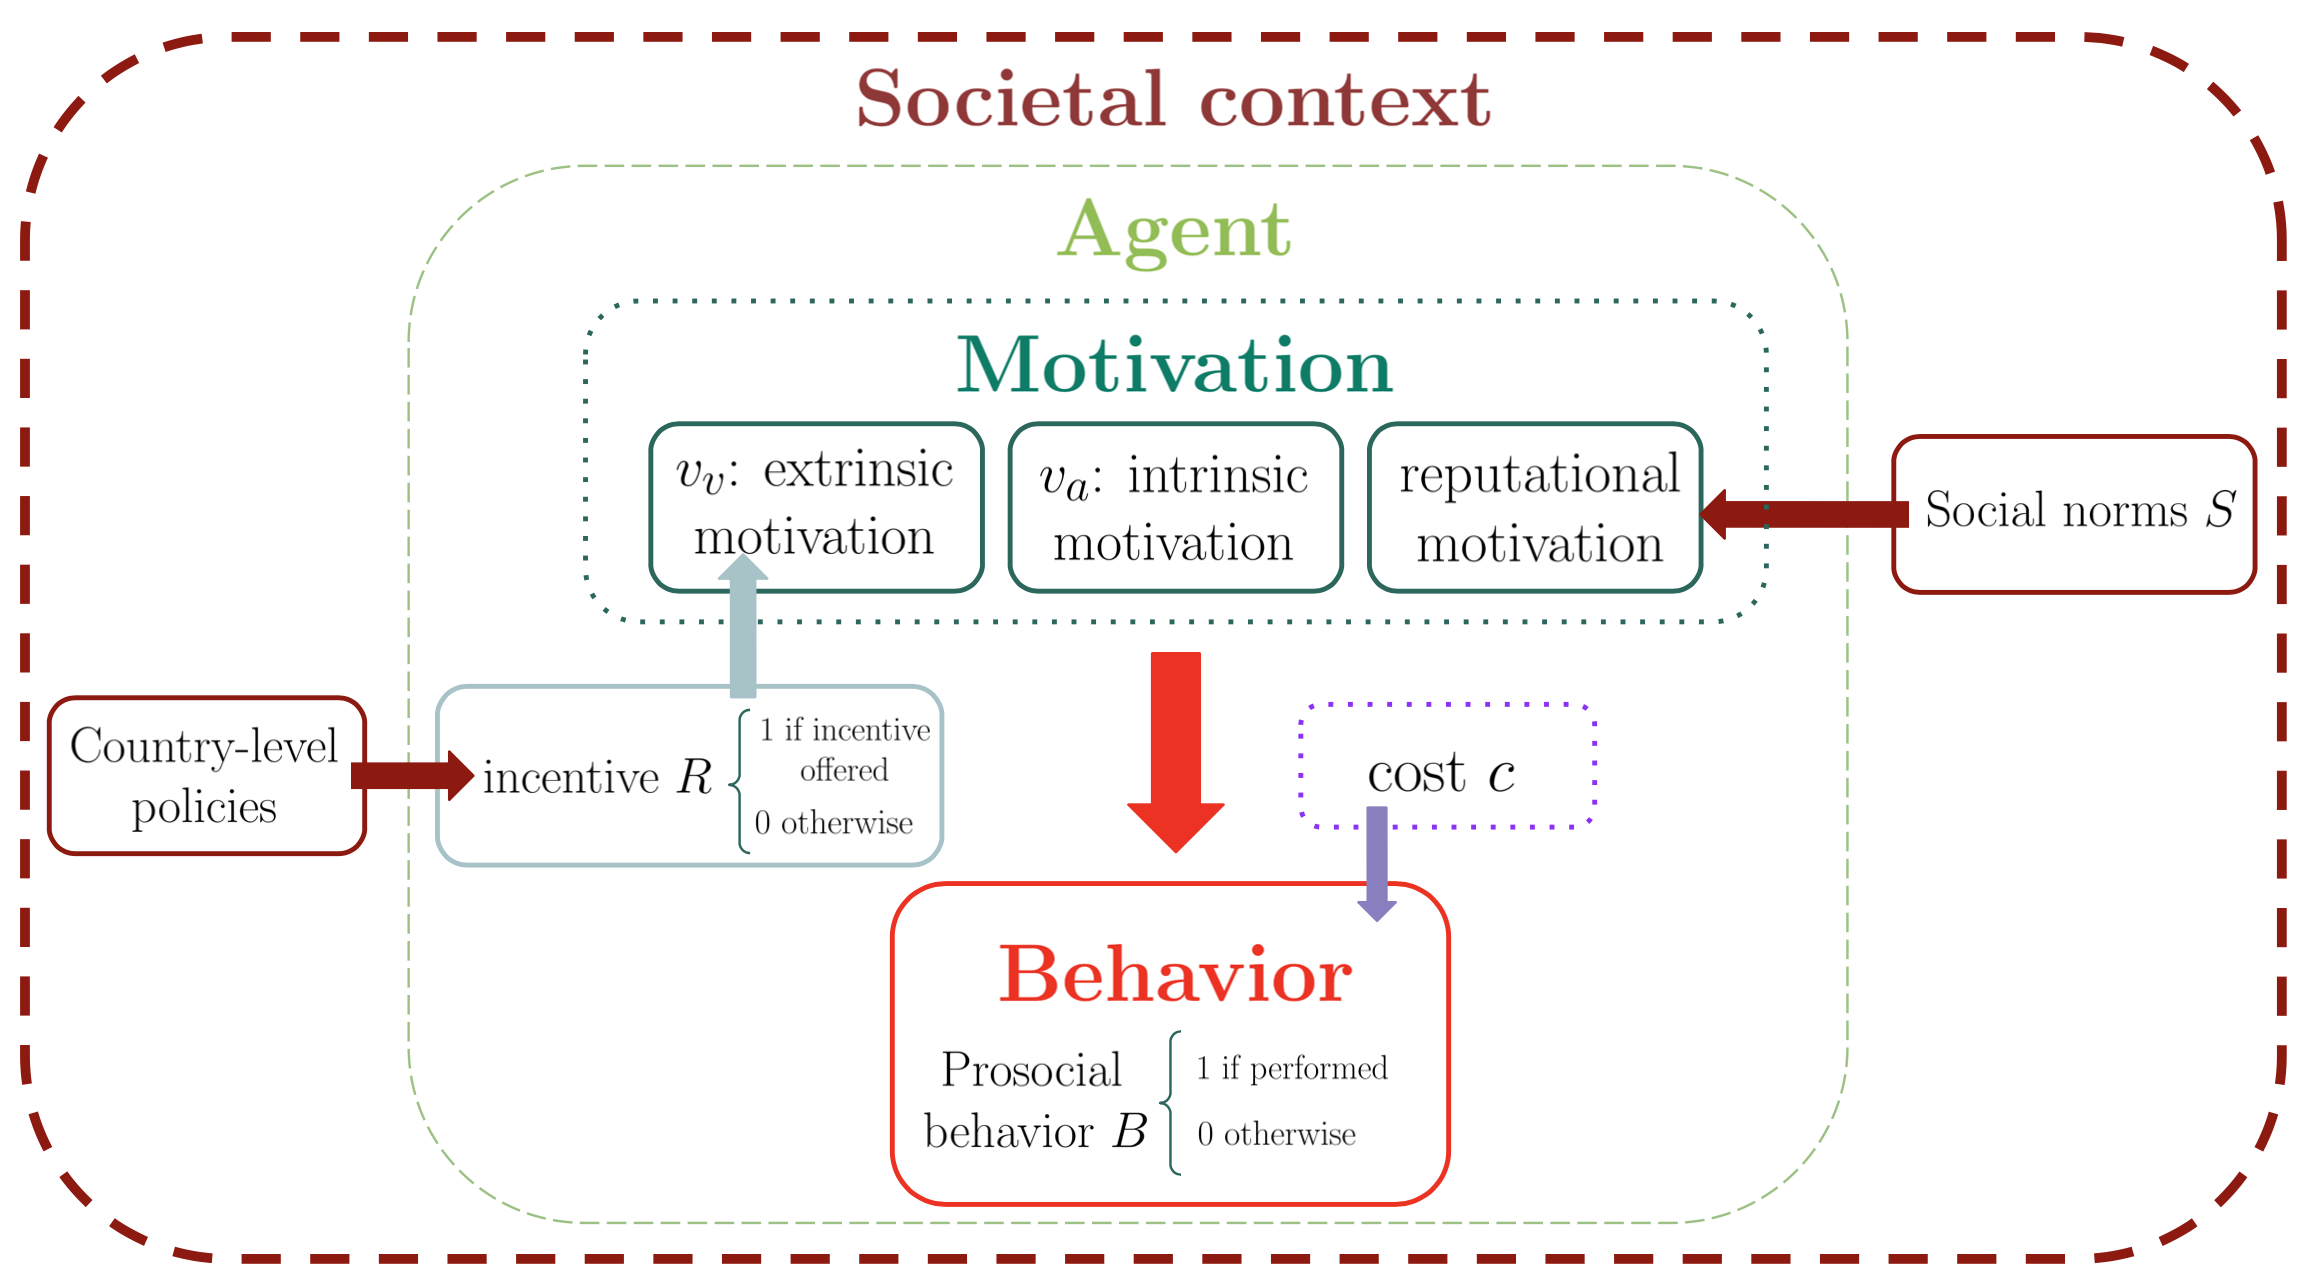
\includegraphics[width=\textwidth]{images/overview.png}
    \caption{Overview of concepts and theoretical framework. Agents are embedded in societal contexts, which shapes the policies for providing incentives, as well as the social norms that govern the reputational outcome of a given behavior. An agent’s behavior is dependent on his motivation, that is (a) intrinsic motivation, (b) extrinsic motivation (in case incentives are provided), and (c) reputational motivation (based on the social norms prevalent in the societal context), as well as his costs.}
    \label{fig:overview}
\end{figure}

This work aims to contribute several novel insights: Firstly, we modify the conceptualization of reputational motivation, and extend it by taking into account social norms. Instead of making an assumption about the reputational outcome of certain behaviors, we elicit social norms empirically and use this as a proxy for reputational motivation. This is possible because we test the model in a cross-societal context, where we are able to exploit variation in social norms. Secondly, we apply this adapted theory of prosocial behavior to the “ultimately altruistic” act of blood donation, which provides a real-world test of our theoretical description of prosocial behavior and adds to a better understanding of the external validity of the model.

The current paper is structured in the following way: Firstly, we formally specify our model, building on the model developed by \cite{benabou_incentives_2006}. Within simulations we illustrate predictions of the model given different parameter settings. Then, we describe our methodology, including our dataset and operationalization of the variables in the model. Next, we present the results of hierarchical mixed effects models. Lastly, we conclude and offer further directions for future research.

\section{The Model}

We base our model on the model of prosociality by \cite{benabou_incentives_2006}, and focus on binary prosocial activities that can either be performed or not (e.g., voting, donating blood; the model can generally also be applied to continuous contexts, e.g. charity donations, see \cite{benabou_incentives_2006}). In the beginning of this model description we concentrate on the isolated agent; That is, we ignore the societal context in which agents are nested (see Fig.  \ref{fig:model_IM_EM}) until later parts of this section. Moreover, we retrace the steps of \cite{benabou_incentives_2006} and thus introduce the reputational motivation component only after summarizing the effect of intrinsic and extrinsic motivation as the so called \textit{direct benefit} associated with the behavior.

\paragraph{Intrinsic and extrinsic motivation}

Suppose an agent A with intrinsic motivation $v_{a} \in [0,1]$ and extrinsic motivation $v_{v} \in [0,1]$ must decide between engaging in a prosocial behavior B, which may be associated with extrinsic reward $R \in \{0,1\}$ \footnote{textit{Incentives} are extrinsic rewards that motivate behavior, and thus the two terms are here used interchangeably. For convenience, we take extrinsic rewards to be a binary variable, but the model can easily be modified to include continuous reward values.} and cost $c$. The direct benefit associated with the behavior is then the following: 

$$ \mbox{\textit{direct benefit}} = B * (v_{a} + v_{v} * R) - B * c $$

In the absence of extrinsic rewards (i.e., R = 0), only intrinsic motivation $v_{a}$ and personal cost $c$ determine whether the prosocial action is performed. Personal cost here refers to the individual-level cost associated with the activity, for instance in terms of time, money, and resources. Although costliness of the behavior varies across individuals, it is also conceivable that some activities are highly costly for many people (such as donating a kidney) and are thus performed only by very few who have exceptionally high intrinsic motivation and relatively low cost. On the other hand, some behaviors may be associated with relatively low costs for most people (such as helping someone who tripped and fell) and are therefore performed by most people who have sufficiently high intrinsic motivation. Assuming that the prosocial behavior is performed if \textit{direct benefit} is greater for B = 1 than for B = 0, the effect of cost \footnote{For illustrative purposes, cost is here assumed to be the same for all individuals. This will however not be a constraint in our model, where cost will instead be able to vary across people.} is illustrated in Fig.  \ref{fig:model_IM_EM}: In the first row we can see the effect of varying the cost of the prosocial activity in the absence of incentives. In the upper leftmost facet, most people engage in the behavior (red), because relatively low levels of intrinsic motivation suffice to engage in the relatively uncostly behavior. On the upper rightmost facet is the other extreme, where only the most highly intrinsically motivated members of society perform the prosocial action given the high associated costs.

\begin{figure}[h]
    \centering
    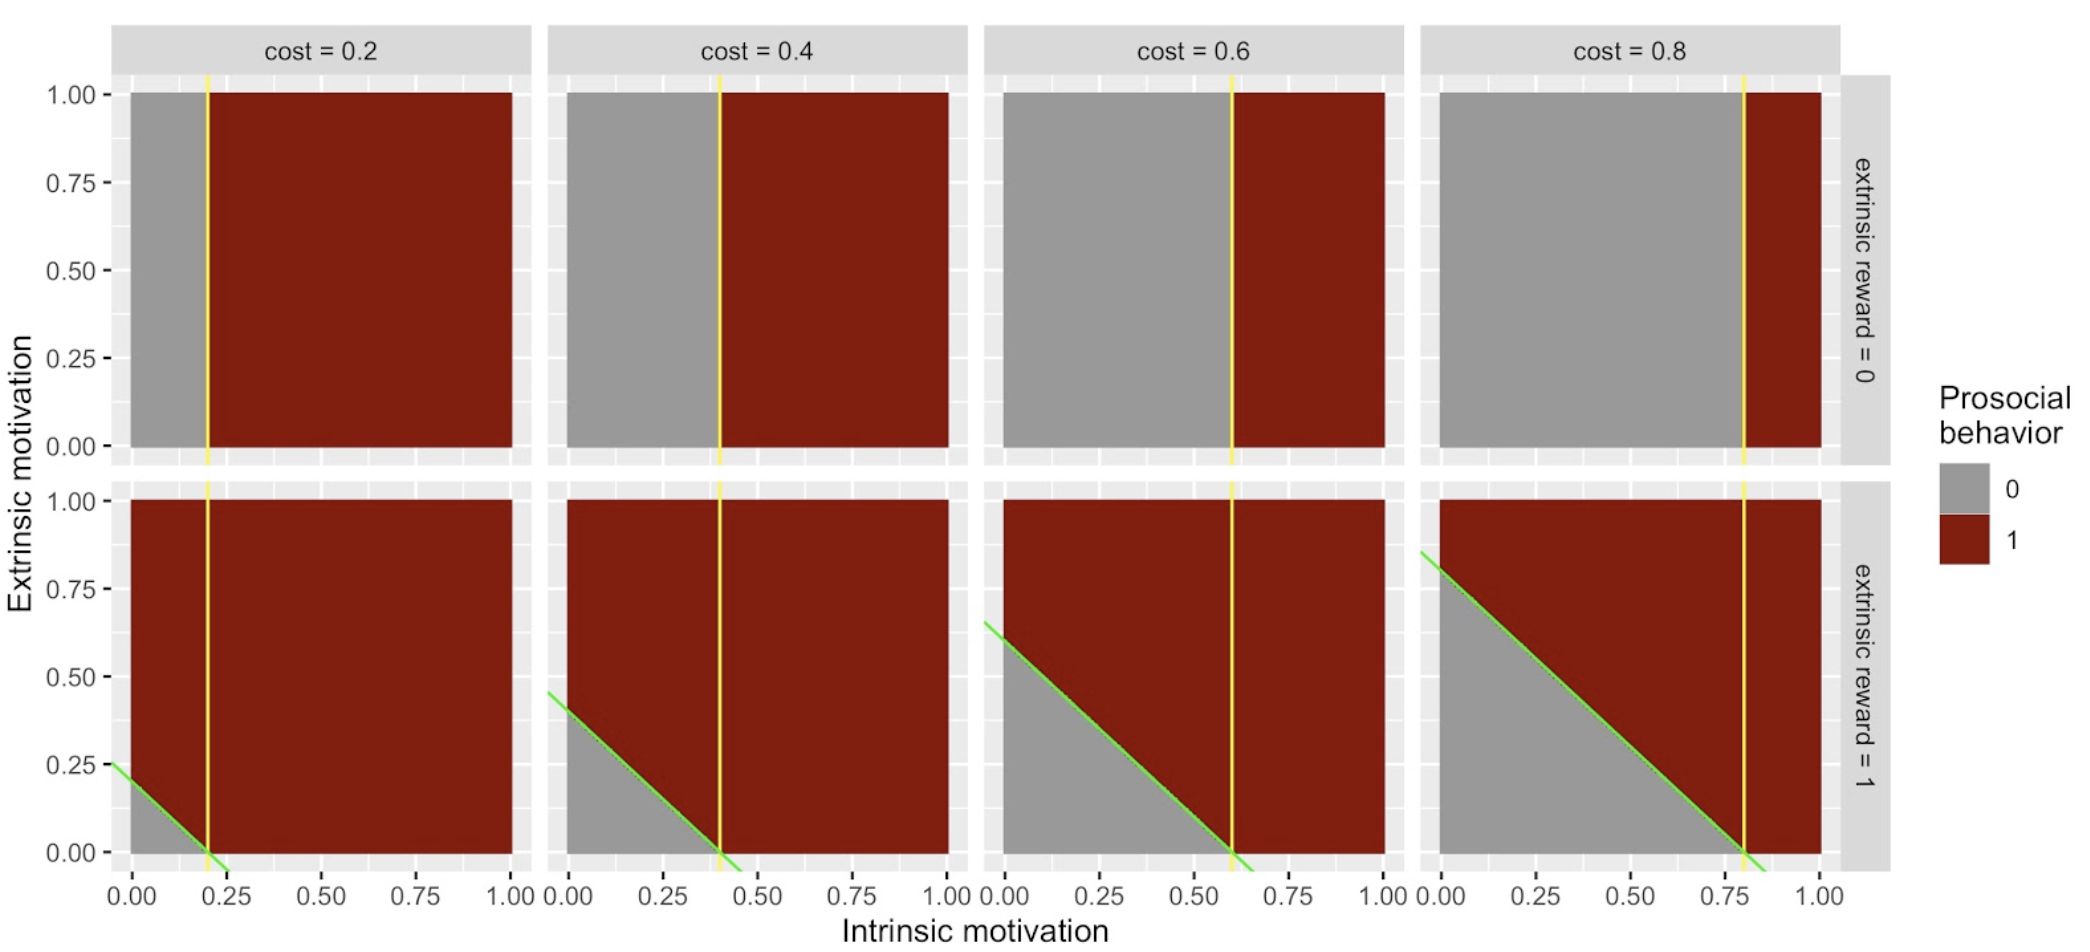
\includegraphics[width=\textwidth]{images/model_IM_EM.png}
    \caption{Visualization of the effects of varying cost of the behavior (as depicted in the four columns) and the presence of incentives (as depicted in the two rows) for individuals varying in intrinsic and extrinsic motivation. The first row illustrates that in the absence of extrinsic rewards, intrinsic motivation and cost govern whether a behavior is performed (yellow line; For example, if cost is 0.4 and incentive = 0, then those individuals whose intrinsic motivation is greater than 0.4 perform the prosocial behavior, irrespective of their extrinsic motivation). In the second row, where incentives are provided, the line dividing those taking the action versus not (green line) shifts counterclockwise: More people engage in the prosocial behavior, because sufficiently extrinsically motivated individuals also engage in the behavior (For example, if cost is 0.6 and incentive = 1, those individuals whose intrinsic motivation is greater than 0.6 perform the prosocial behavior, as in the first row, and \textit{additionally} those individuals whose sum of extrinsic and intrinsic motivation is greater than 0.6 perform the prosocial behavior.).}
    \label{fig:model_IM_EM}
\end{figure}

When incentives are offered, the decision to perform the prosocial behavior is governed both by extrinsic and intrinsic motivation (as well as costs). This results in a higher total number of individuals that join in performing the behavior, because they are motivated by the extrinsic reward. The bottom row in Fig. \ref{fig:model_IM_EM} shows this effect: the dividing line between those who engage in the prosocial behavior and those who do not virtually tips over toward the left side, as individuals with insufficient intrinsic motivation but some extrinsic motivation now choose to perform the behavior as well. 

\paragraph{Reputational motivation}

\cite{benabou_incentives_2006} furthermore incorporate \textit{reputational motivation} in the model (i.e., the third motivational component besides intrinsic and extrinsic motivation, as depicted in Fig. \ref{fig:model_IM_EM}), which is dependent on $VIS$, the visibility of the action (i.e., to what extent the behavior is performed in private vs. public), as well as $pref_{v_{a}}$ and $pref_{v_{v}}$, the individual’s preference to appear intrinsically motivated and not extrinsically motivated, respectively. Most importantly, reputational motivation is dependent on the \textit{expected value} of an individual’s intrinsic and extrinsic motivation given their behavior and the extrinsic reward associated with the behavior. In Benabou and Tirole’s (2006) model the expected value of extrinsic motivation $E(v_{v})$ is a \textit{cost} whereas the value of intrinsic motivation $E(v_{a})$ is a \textit{gain}. Reputational motivation is defined as follows:

$$ \mbox{\textit{reputational benefit}} =  VIS[pref_{v_{a}} * E(v_{a} | R, B) - pref_{v_{v}} * E(v_{v} | R, B)] $$

As the authors point out, the first component of \textit{reputational benefit} (namely $VIS * pref_{v_{a}} * E(v_{a} | R, B)$; of which the driving factor is the expected value of intrinsic motivation $E(v_{a} | R, B))$ has the same effect when R = 1 and R = 0: Individuals who engage in the prosocial activity always have a higher expected intrinsic motivation than individuals who do not behave prosocially \citep{benabou_incentives_2006}. This holds irrespective of whether an extrinsic reward is offered. That is,

	$$E(v_{a} | R = 0, B = 1) \mathbin{\color{red}>} E(v_{a} | R = 0, B = 0)$$ 
	and
		$$E(v_{a} | R = 1, B = 1) \mathbin{\color{red}>} E(v_{a} | R = 1, B = 0) $$

The same does not hold for the cost associated with higher expected extrinsic motivation: Here it is in fact the case that in the presence of incentives, the expected value for extrinsic motivation is higher for individuals engaging in the prosocial activity than not, and this is not the case when there are no incentives provided. That is,

	$$E(v_{v} | R = 0, B = 1) \mathbin{\color{red}=} E(v_{v} | R = 0, B = 0)$$
	and
		$$E(v_{v} | R = 1, B = 1) \mathbin{\color{red}>} E(v_{v} | R = 1, B = 0) $$

In other words, when no extrinsic rewards are provided, there is no information about the value of extrinsic motivation. But when extrinsic rewards are offered, the expected value of extrinsic motivation of prosocially behaving individuals is higher than that of non-prosocially behaving individuals.

\paragraph{The full model}

We follow \cite{benabou_incentives_2006} in proposing an additive effect of the direct (equation [1]) and reputational (equation [2]) benefits of the behavior. That is, an agent A solves the following equation when deciding whether to engage in the prosocial behavior: 

$$Max		\{ \mbox{\textit{direct benefit + reputational benefit}} \}, B \in \{0,1\}$$

In order to derive the predictions of the model for behavior, let us consider which benefits apply to which behavioral action: \textit{direct benefit} applies only to actions taken. That is, if B = 0, \textit{direct benefit} is zero. If B = 1, \textit{direct benefit} is equal to equation [1]. As a consequence, when only taking into account \textit{direct benefit} and not \textit{reputational benefit}, prosocial behavior is performed if \textit{direct benefit} > 0.

The same is not true for reputational benefit, as the expected values of intrinsic and extrinsic motivation are defined irrespective of B. In the 2x2 matrix below the total benefits (direct benefit + reputational benefit) associated with choosing not to perform the behavior (B = 0, first column) or performing the behavior (B = 1, second column) are presented; agent A must weigh his benefits given incentives being absent (R = 0, first row) or present (R = 1, second row):


\begin{tabular}{c|c|c}
& B = 0 & B = 1 \\
\hline
R = 0 & $E(v_{a} | R = 0, B = 0) - E(v_{v} | R = 0, B = 0)$ & $v_{a} - c +
E(v_{a} | R = 0, B = 1) - E(v_{v} | R = 0, B = 1)$\\
\hline
R = 1 & $E(v_{a} | R = 1, B = 0) - E(v_{v} | R = 1, B = 0)$ & $v_{a} + v_{v} - c +
E(v_{a} | R = 1, B = 1) - E(v_{v} | R = 1, B = 1)$ \\
\end{tabular}

Although the precise numerical values of expected intrinsic and extrinsic motivation depend on the nature of the prosocial activity (such as the cost $c$ of the behavior), we do have some insights about the expected values. Firstly, $E(v_{a})$ is always higher when B = 1 than when B = 0 (see [3]). When A weights his benefits for B = 0 versus B = 1, $E(v_{a})$ will thus always draw him to perform the prosocial behavior: B = 1. As \cite{benabou_incentives_2006} have mentioned, $E(v_{a})$ is thus not very informative, and the major contribution of the reputational motivation component does not come from a gain in $E(v_{a})$ but instead from a cost of $E(v_{v})$: From [4] we see that in the case of R = 0, $E(v_{v})$ is equivalent for both cases where the action is performed or not. When A weighs the benefits associated with choosing B in the absence of incentives (R = 0), $E(v_{v})$ will therefore cancel out on both sides. However, the same does not hold for the case when R = 1. In this case, $E(v_{v})$ is larger for B = 1 than for B = 0. This means that the agent faces an additional cost when performing the behavior in the presence of extrinsic rewards, and this may tip him over to not engaging in the action. This cost of higher expected extrinsic motivation $E(v_{v})$ thus plays a central role in implementing the negative effect of incentives on prosocial behavior.

From these considerations we can approximate that under Benabou and Tirole’s (2006) model\footnote{As argued above, we take the effect of expected intrinsic motivation to be negligible. It can be included in the model as the positive difference between $E(v_{a} | B = 1)$ and $E(v_{a} | B = 0)$. As its sign is necessarily positive (see [3]), including this term would additionally encourage prosocial behavior. We also hold $VIS$ and $pref_{v_{v}}$ constant at 1, but these can easily be incorporated by adding them to the expected extrinsic motivation term: $E(v_{v} | B = 1) * VIS * pref_{v_{v}}$.}, prosocial behavior B is performed if the following holds:

	$$v_{a} - c + R * (v_{v}  -  E(v_{v} | B = 1, R = 1) )  \mathbin{\color{red}> 0}$$

Thus, an agent A weighs his intrinsic motivation $v_{a}$, the cost of donation $c$, and, in case incentives R are provided, his extrinsic motivation $v_{v}$ and cost of expected extrinsic motivation $E(v_{v})$.

\paragraph{Modification: Incorporating social norms}
	
Reputational motivation, which is conceptualized thus far as the cost related to expected extrinsic motivation, relies on the assumption that humans are generally motivated not to appear extrinsically motivated (i.e., expected extrinsic motivation always represents a reputational cost to an agent, unless the individual’s strength of preference not to appear extrinsically motivated is zero, or in case the visibility of the action is zero). We put this assumption into question by introducing our key modification to the model: We take reputational motivation to stem not from a cost of expected extrinsic motivation per se, but to be determined by the social norms governing the provision of extrinsic rewards for a given prosocial behavior. We call this social norm variable $S$, and define it as the \textit{sum of reputational costs and benefits as dictated by the prevalent social norms} that are associated with a given behavior. From this follows our conceptualization of reputational benefit:

$$\mbox{\textit{reputational benefit}} = B * R * S \mbox{ , where  } S \in [-1,1]$$

We thereby assume that the overall reputational value (i.e., cost \textit{or} benefit) is determined by the specific set of social norms that are prevalent in an individual’s environment. Depending on the social environment, the net effect of social norms regarding incentives can be \textit{positive} (i.e., $S > 0$) or \textit{negative} ($S < 0$).

Figure \ref{fig:model_SOC} illustrates the effect of the social norms variable S on prosocial behavior. The first row shows that a \textit{negative} value of S shifts the diagonal line dividing those taking the action versus not (green line) toward the right on the x-axis. This has as a result that the extrinsic reward motivates some highly extrinsically motivated and moderately intrinsically motivated individuals to perform the behavior (i.e., those with lower intrinsic motivation than the yellow threshold line yet still above the green threshold line), but it also leads some individuals (who are highly intrinsically motivated and not highly extrinsically motivated) to stop performing the behavior. This is due to them carrying a reputational cost that comes about by social norms that characterize it as “bad” that the given prosocial behavior is performed while receiving an extrinsic reward. The first row in Fig. \ref{fig:model_SOC} describes precisely the pattern which \cite{benabou_incentives_2006} predicted and captured in their model as the cost of expected extrinsic motivation.

\begin{figure}[h]
    \centering
    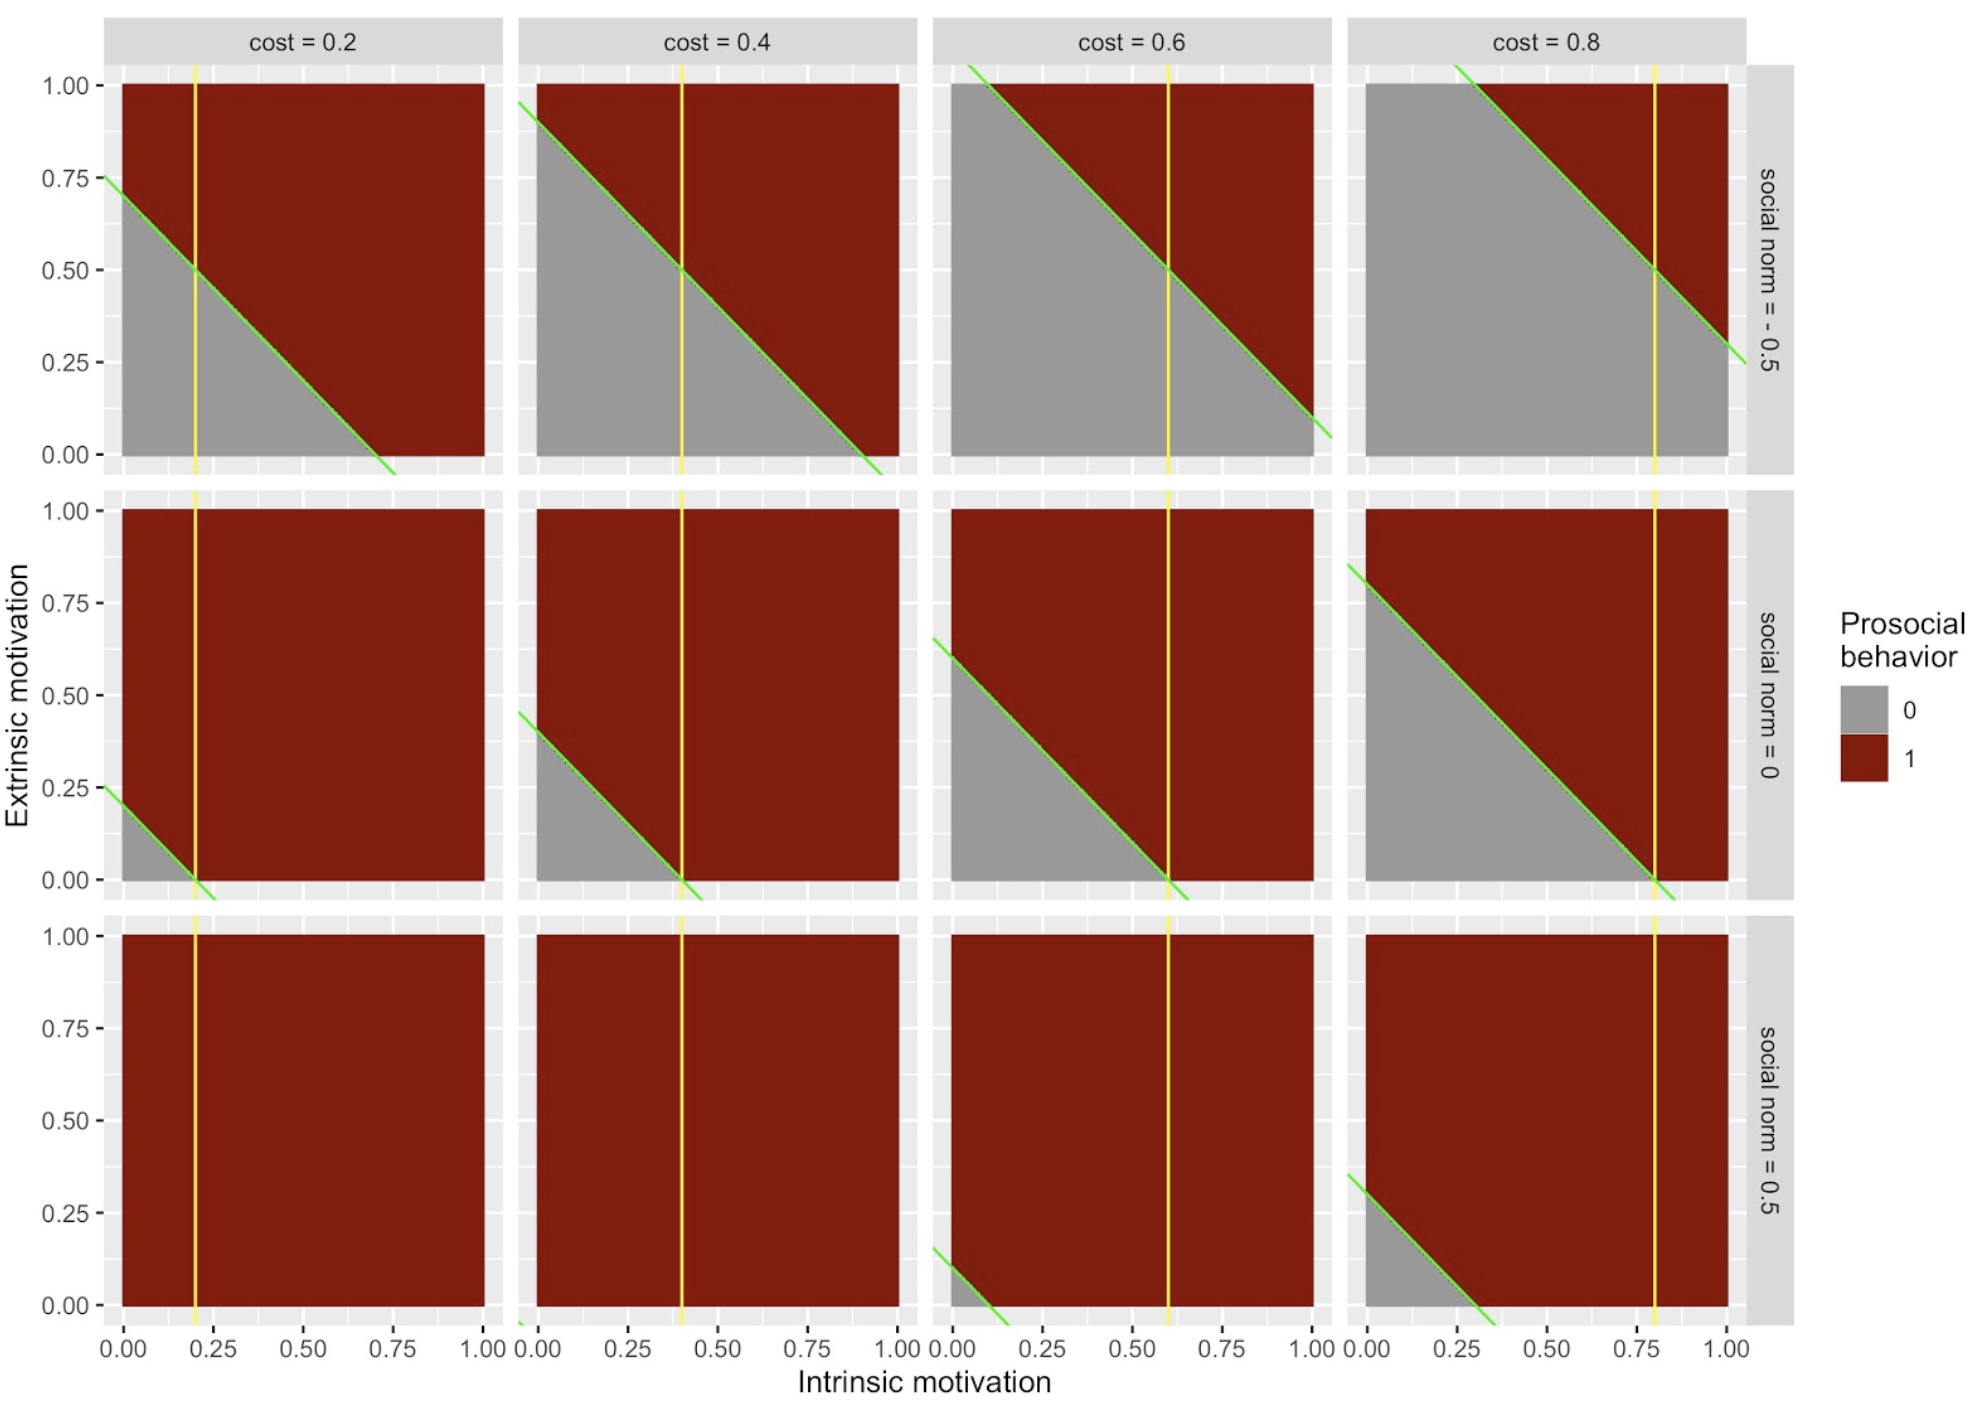
\includegraphics[width=\textwidth]{images/model_SOC.png}
    \caption{In the presence of extrinsic rewards, the value of the social norms variable S (where varying values are depicted across the rows) determines the shift on the x-axis of the diagonal line dividing those behaving prosocially versus not (green line; see description in main text).}
    \label{fig:model_SOC}
\end{figure}


The second row of Figure \ref{fig:model_SOC} depicts the scenario where the net effect of social norms is zero. In this case, only extrinsic and intrinsic motivation plays a role (as well as cost), as is the case in the bottom row of Fig. \ref{fig:model_IM_EM}. Lastly, the third row of Fig. \ref{fig:model_SOC} illustrates the effect of a \textit{positive} value of S on prosocial behavior, in which the diagonal threshold line dividing those behaving prosocially versus not (green line) is shifted to the left on the x-axis. In this case, the combined positive effect of intrinsic, extrinsic and reputational motivation leads to high levels of prosocial behavior.

Incorporating our modification into the full model, we thus predict that prosocial behavior B is performed if the following holds:

$$v_{a} - c + R * (v_{v}  + S) \mathbin{\color{red}> 0}$$

In conclusion, we theorize an additive effect of intrinsic and extrinsic motivation, cost, as well as reputational motivation governed by social norms. Hereby, intrinsic motivation and individual-level cost play a role in determining behavior irrespective of rewards; extrinsic motivation and the impact of social norms for incentives only have an effect on prosocial behavior if incentives are provided. 

\section{Materials and Methods}

\paragraph{Participants and procedure}

In order to test our model of prosocial behavior we employ comparative data from the 2014 wave of the Eurobarometer \citep{european_commission_eurobarometer_2014}, combined with a survey about incentive policies among experts in the included European countries. The Eurobarometer (EB) is a repeated cross-sectional survey conducted on representative samples from the European Union (EU) member states. In 2014, the survey was performed in a total of 28 countries. A multi-stage random (probability) sampling design was employed and approximately 1000 face-to-face interviews were completed in each of the countries \footnote{Exceptions are Luxembourg, Cyprus and Malta with 500 interviews each, as well as the United Kingdom with separate samples for Great Britain (1000) and Northern Ireland (300) and Germany with separate samples for former East (500) and West (1000) Germany.}. Respondents were residents of the respective country, had sufficient command of the national language(s), and were 15 years or older. Study protocols were approved by the European Commission and all participants provided informed consent. The expert survey was conducted among specialists from blood collecting institutions who were contacted by email and provided responses either in writing or via a telephone interview\footnote{Incentive data for the Czech Republic, France, and the Netherlands were taken from a recent Vox Sanguinis expert survey on incentives across the globe \citep{zeller_vox_2020}.}.

\paragraph{Operationalization and Variables}

The 2014 round of the Eurobarometer included items on blood donation behavior, motivation to donate, and attitudes regarding incentives for blood donation. An overview of the dependent and independent variables, including the wording of survey items and response ranges, are presented in supplementary Table 1. In the following we describe the operationalization of variables in more detail.

\textbf{Blood donation} The dependent variable in our analyses is blood donation during one's lifetime. Participants in the Eurobarometer were asked whether they have ever donated substances of human origin, among them whole blood. 

\textbf{Intrinsic motivation} Intrinsic motivation is operationalized as the mentioning (yes/no) of an intrinsic motivational factor as a reason why respondents have donated or are willing to donate blood. Intrinsic motivation takes on the value 1 if one of three intrinsic motivational factors are mentioned: (a) to help other people in need, (b) to alleviate shortages of these substances, or (c) to support medical research. 

\textbf{Extrinsic motivation} Extrinsic motivation is operationalized as a set of variables: (a) mentioning (yes/no) of an extrinsic factor to be a reason for donating or being willing to donate blood (namely “to receive something in return for you or your relatives”), (b) the subjective difficulty in paying bills (three levels: Almost never \ never; From time to time; Most of the time), and (c) an indication of lack of financial liquidity as suggested by current employment status\footnote{Note that the lack of current employment can be seen as a source of motivation for financial reward, but the \textit{presence of current employment} can also be seen as a \textit{cost} to donate, because working individuals are more affected by time constraints. This will need to be considered when interpreting the effect of this variable.}. Although lack of current employment and subjective difficulty in paying bills may be related, we include both, because these indicators target partly overlapping but possibly distinct parts of the population that profit from earning extra money on the side: Those who are employed but do not earn enough (and therefore have trouble paying bills) and those who are not employed (such as students and retirees). By taking into account the current financial situation of the respondent, we acknowledge that the utility of monetary rewards is reference-dependent in that it hinges on the current assets of the individual \citep{tversky_loss_1991}. That is, we assume that individuals with lower income experience a higher increase in subjective utility from receiving a set amount of money compared to individuals with higher income \footnote{This is also in line with evidence that financial incentives are viewed more positively by younger donors who typically have fewer financial assets than older donors \citep{glynn_attitudes_2003}.}.

\textbf{Personal cost} Individuals face varying costs and constraints to donating blood. We include two possible factors that independently influence the costliness of donation: (a) time constraints due to child care \cite[i.e., parents of small children may perceive time constraints to donate; ][]{piersma_blood_2019}, and (b) travel costs due to rural living (i.e., rural areas have a smaller density of blood collection organizations (BCOs) and therefore residents from these areas face greater costs in both financially and in terms of travel time).

\textbf{Social norms} Social norms by definition apply to the (societal) group level, and we thus construct the social norm variable by aggregating responses of individual participants regarding the social acceptability of receiving incentives for blood donation for the 28 European countries. We calculate the social norm variable both for \textit{financial} incentives and \textit{time} incentives. The aggregated variable ranges from 0 (i.e., 0% or respondents find cash/time incentives acceptable) to 1 (i.e., 100% or respondents find cash/time incentives acceptable).

\textbf{Socio-demographic controls} Finally, we control for important confounding factors. Firstly, we take into account the age of respondents, as our dependent variable \textit{blood donation during lifetime} is dependent on years lived (i.e., older individuals have had more time in their life to have ever donated). Moreover, we include gender, education, and partner status as socio-demographic control variables, as these variables were shown to be related to propensity to donate in previous studies (although there are some inconsistent findings between studies, for example related to gender; see \cite{piersma_individual_2017} for a recent review on donor demographics).

\textbf{Incentives} Incentives are rewards that are provided to donors with the goal of motivating donation.  For blood donation, large differences in the provision of incentives exist across countries. We constructed a database of incentives offered to donors in different European countries by conducting a survey among experts (either in interview or written form). Experts were largely employees from national blood collection agencies and were consulted about the type and value of incentives provided in their country. We explicitly asked experts not to report small-value incentives (as it is quite common that donors are given small rewards such as t-shirts, mugs or towels), as we are only interested in high-value (non-symbolic) incentives. Based on expert responses we constructed two country-level incentive variables, one for financial incentives (i.e., cash or other incentives with financial value, for example tax deduction; the incentive should be high-value, i.e., at least 10 Euro) and the other for time incentives (i.e., time off work). Financial incentives were categorized into: (a) Financial incentives offered by \textit{no} blood operators, (b) \textit{some} blood operators offer financial incentives but others do not, and (c) all blood operators offer financial incentives. Time incentives also had three levels: (a) Time incentives offered by \textit{no} blood operators, (b) time incentives are offered \textit{dependent on the employer} (i.e., in some countries only some employers offer donors to donate during work hours, often this was the case for government employees), and (c) time incentives are offered \textit{independent of the employer}. Incentives enter the model in interaction terms with both extrinsic motivation and social norms. The items from the expert survey as well as an overview of the incentive database is provided in the appendix.


\paragraph{Statistical analysis}

\textbf{Exclusion criteria} Respondents who are younger than 18 years are excluded, because their age would not allow them to donate blood in most EU countries. Although individuals above the age of 65 are usually not eligible anymore to donate blood, we include these subjects in our sample, because our dependent variable is blood donation \textit{during the lifetime}. 

\textbf{Multilevel modeling} We employ logistic multilevel mixed effects models for all main analyses, where individuals are nested in countries. This method allows us to include individual-level variables (e.g., intrinsic motivation) and country-level variables (e.g., social norms regarding incentives) as fixed effects, as well as allowing the intercept to vary by country. The estimation technique is maximum likelihood; Missing values are handled by means of listwise deletion. 

In order to find the best fitting model while avoiding overfitting, we take a procedural approach of implementing nested models. That is, we add the independent variables to the baseline model (i.e., the intercept-only model which only includes the random intercept) in a stepwise manner and compare the resulting model fit with AIC. To this end we first estimate the intercept-only model (the “empty model” without predictors), then add the demographic control variables, and finally incorporate our predictors of interest. We run separate models for financial and non-financial (time) incentives; the predictors of interest for the former models are intrinsic motivation, extrinsic motivation, cost, social norms regarding financial incentives, and financial incentives, whereas the key predictors of the latter models are intrinsic motivation, extrinsic motivation\footnote{Extrinsic motivation for time incentives is re-operationalized such that it captures motivation for the extrinsic reward of \textit{time}. As for financial incentives, the mentioning of an extrinsic motivational factor (i.e., getting something in return) is one measure of extrinsic motivation. The other measure for extrinsic motivation for time is employment, because individuals who are employed should be motivated more by getting time off work than those unemployed.}, cost, social norms regarding time incentives, and time incentives. 

Moreover, we test for the significance of the random component of the intercept-only model by performing log-likelihood-ratio tests of models with and without random intercepts for country.

\textbf{Robustness checks} As the \textit{intrinsic motivation} item (i.e., whether respondents are motivated by intrinsic factors) and one of the \textit{extrinsic motivation} items (i.e., whether respondents are motivated by extrinsic factors) was only asked to those who have either donated in the past, or who are willing to donate in the future, by design respondents who did not respond to these items are non-donors. Therefore we have a bias in these variables, and it is necessary to check for the robustness of effects for these two indicators. We thus additionally run all the analyses above excluding those respondents who have not answered these two items. 

\section{Results}

We present the results in three steps: first, we present descriptives and the analysis of random effects and demographics. Then we report the findings related to intrinsic and extrinsic motivation to donate blood, the effect of social norms, and how this interacts with (financial) incentives; and finally we sketch the results from analyses pertaining to non-financial incentives.

\paragraph{Blood donation in Europe}

Overall, 38.4\% (n = 10195\footnote{The supplementary material contains information on exclusion of respondents.}) of all included respondents have ever donated blood. This varied substantially across countries (see Fig. \ref{fig:map_BD}): Donation rates range from 22.8\% of respondents from Portugal having ever donated blood to 52.9\% of respondents from France having donated blood. Table \ref{table:1} displays descriptives of demographic variables and predictors of interest. Figure \ref{fig:map_descr} further displays the geographic distribution of the predictors of interest in our models, which also showed substantial variation across countries (intrinsic motivation: ${X}^2(27) = 1501.5, p < 0.001$; extrinsic motivation: ${X}^2(27)= 408.58, p < 0.001$; social norms regarding financial incentives: ${X}^2(27) = 1970.7, p < 0.001$). Notably, levels of intrinsic motivation to donate (see \ref{fig:map_descr}A) were high across all countries (country-level means ranging from 60.2\% in Bulgaria to 92.5\% in Sweden), albeit higher in Western and Northern European countries compared to Eastern European countries. In contrast, mentioning the extrinsic factor “getting something in return” as motivation to donate was relatively rare (see \ref{fig:map_descr}B; country-level means range from 1.8\% in Italy to 15.6\% in Slovakia). The social norm variable regarding the acceptability of financial incentives for donating blood (see \ref{fig:map_descr}C; values range from 2.2\% in Cyprus to 39.3\% in Bulgaria) also varied widely across the European Union with virtually no acceptance of financial incentives in countries such as Spain, Italy and the United Kingdom, but higher levels of approval in Eastern and Central European countries such as Austria, Bulgaria, the Czech Republic and Latvia. Lastly, the expert survey revealed that only few European countries are offering high-value financial incentives for whole blood: In Bulgaria, the Czech Republic, Poland, and Portugal all blood operators offer high-value incentives to donors. In Germany, some blood operators offer incentives (i.e., hospital-based blood operators) whereas others (i.e., the Red Cross) do not.



\begin{figure}[h]
    \centering
    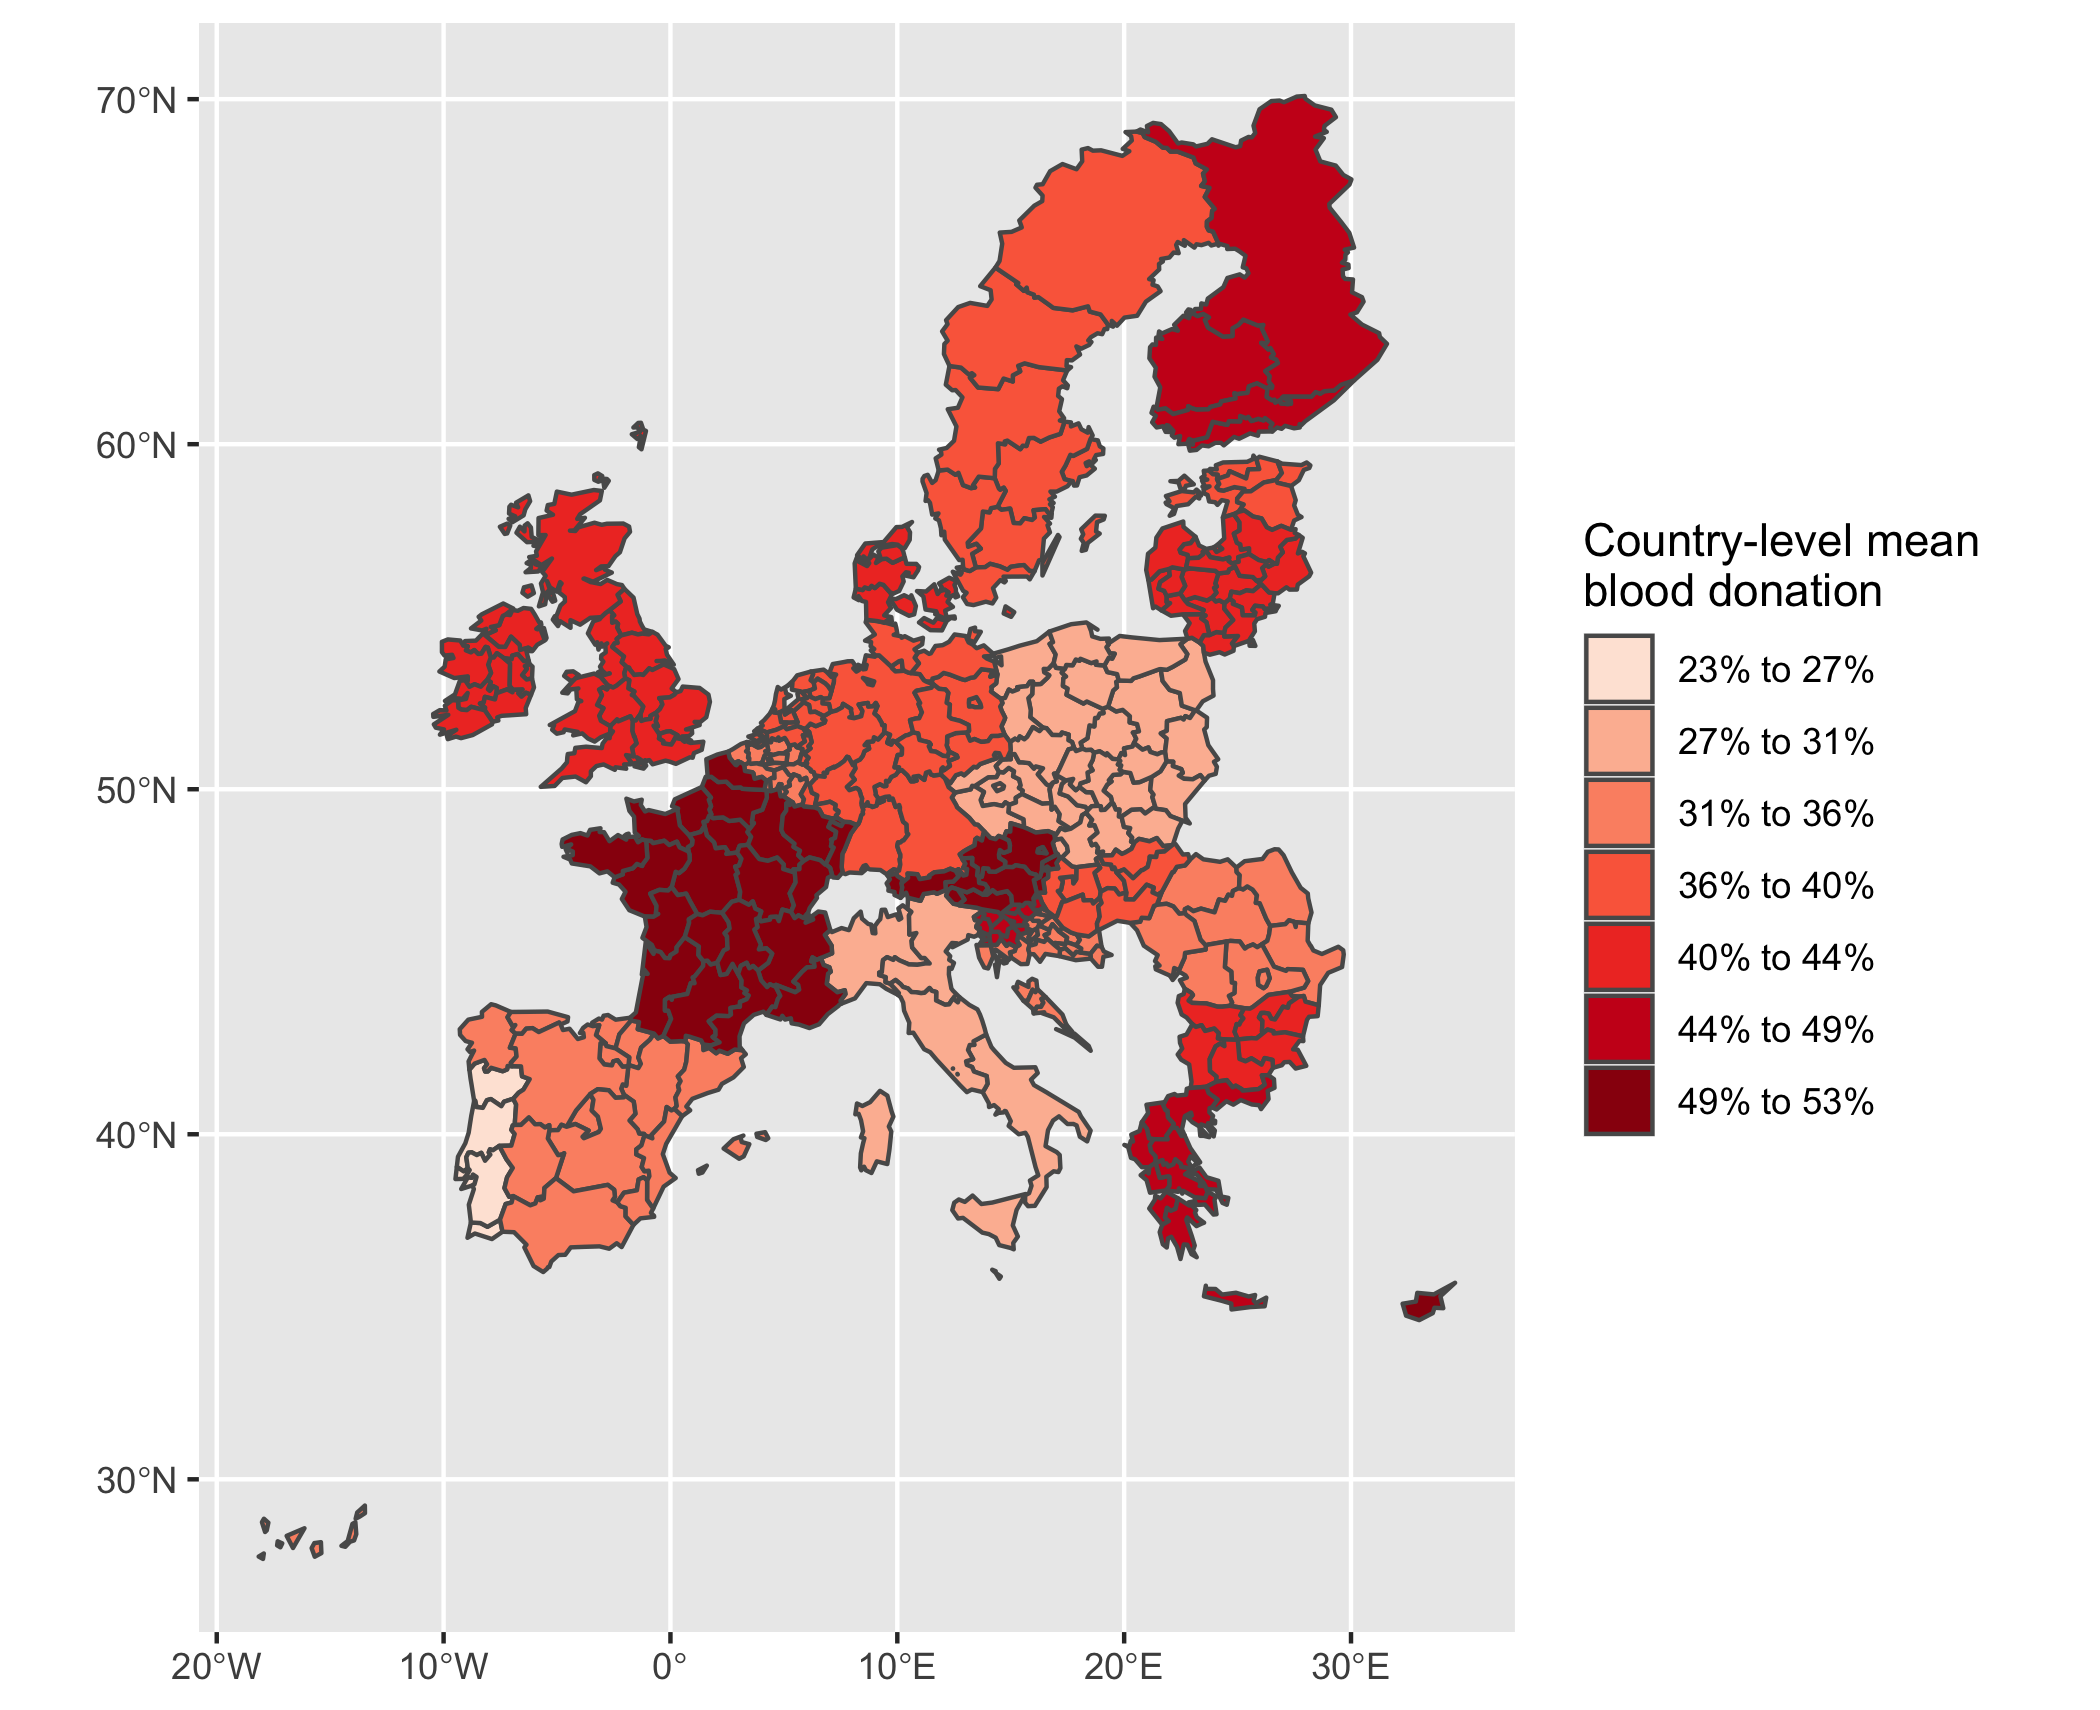
\includegraphics[width=0.9\textwidth]{images/map_BD.png}
    \caption{Country-level mean levels of blood donation.}
    \label{fig:map_BD}
\end{figure}


A log-likelihood test comparing the intercept-only model with the intercept-only model that allows the intercept to vary per country provided strong evidence that including the random intercept component is justified (${\chi}^2(1)=501.79, p < 0.001$). Adding demographics to the model improved the model fit further ($AIC_{demo} = 33097.4 < AIC_{intercept-only} = 34848.6$). As expected given that our dependent variable is blood donation \textit{during the lifetime}, older respondents were more likely to have donated ($b = 0.166, p < 0.001$). The other socio-demographic control variables were also significantly related to blood donation in the following manner: male ($b = -0.471, p < 0.001$) and more educated respondents (full-time education until 16-19 years: $b = 0.395, p = 0.005$; full-time education until 20 years or more: $b = 0.697, p < 0.001$), and those living with a partner ($b = 0.129, p < 0.001$) were more likely to have donated blood during their lifetime.

\begin{figure}
\begin{subfigure}{.48\textwidth}
  \centering
  % include first image
  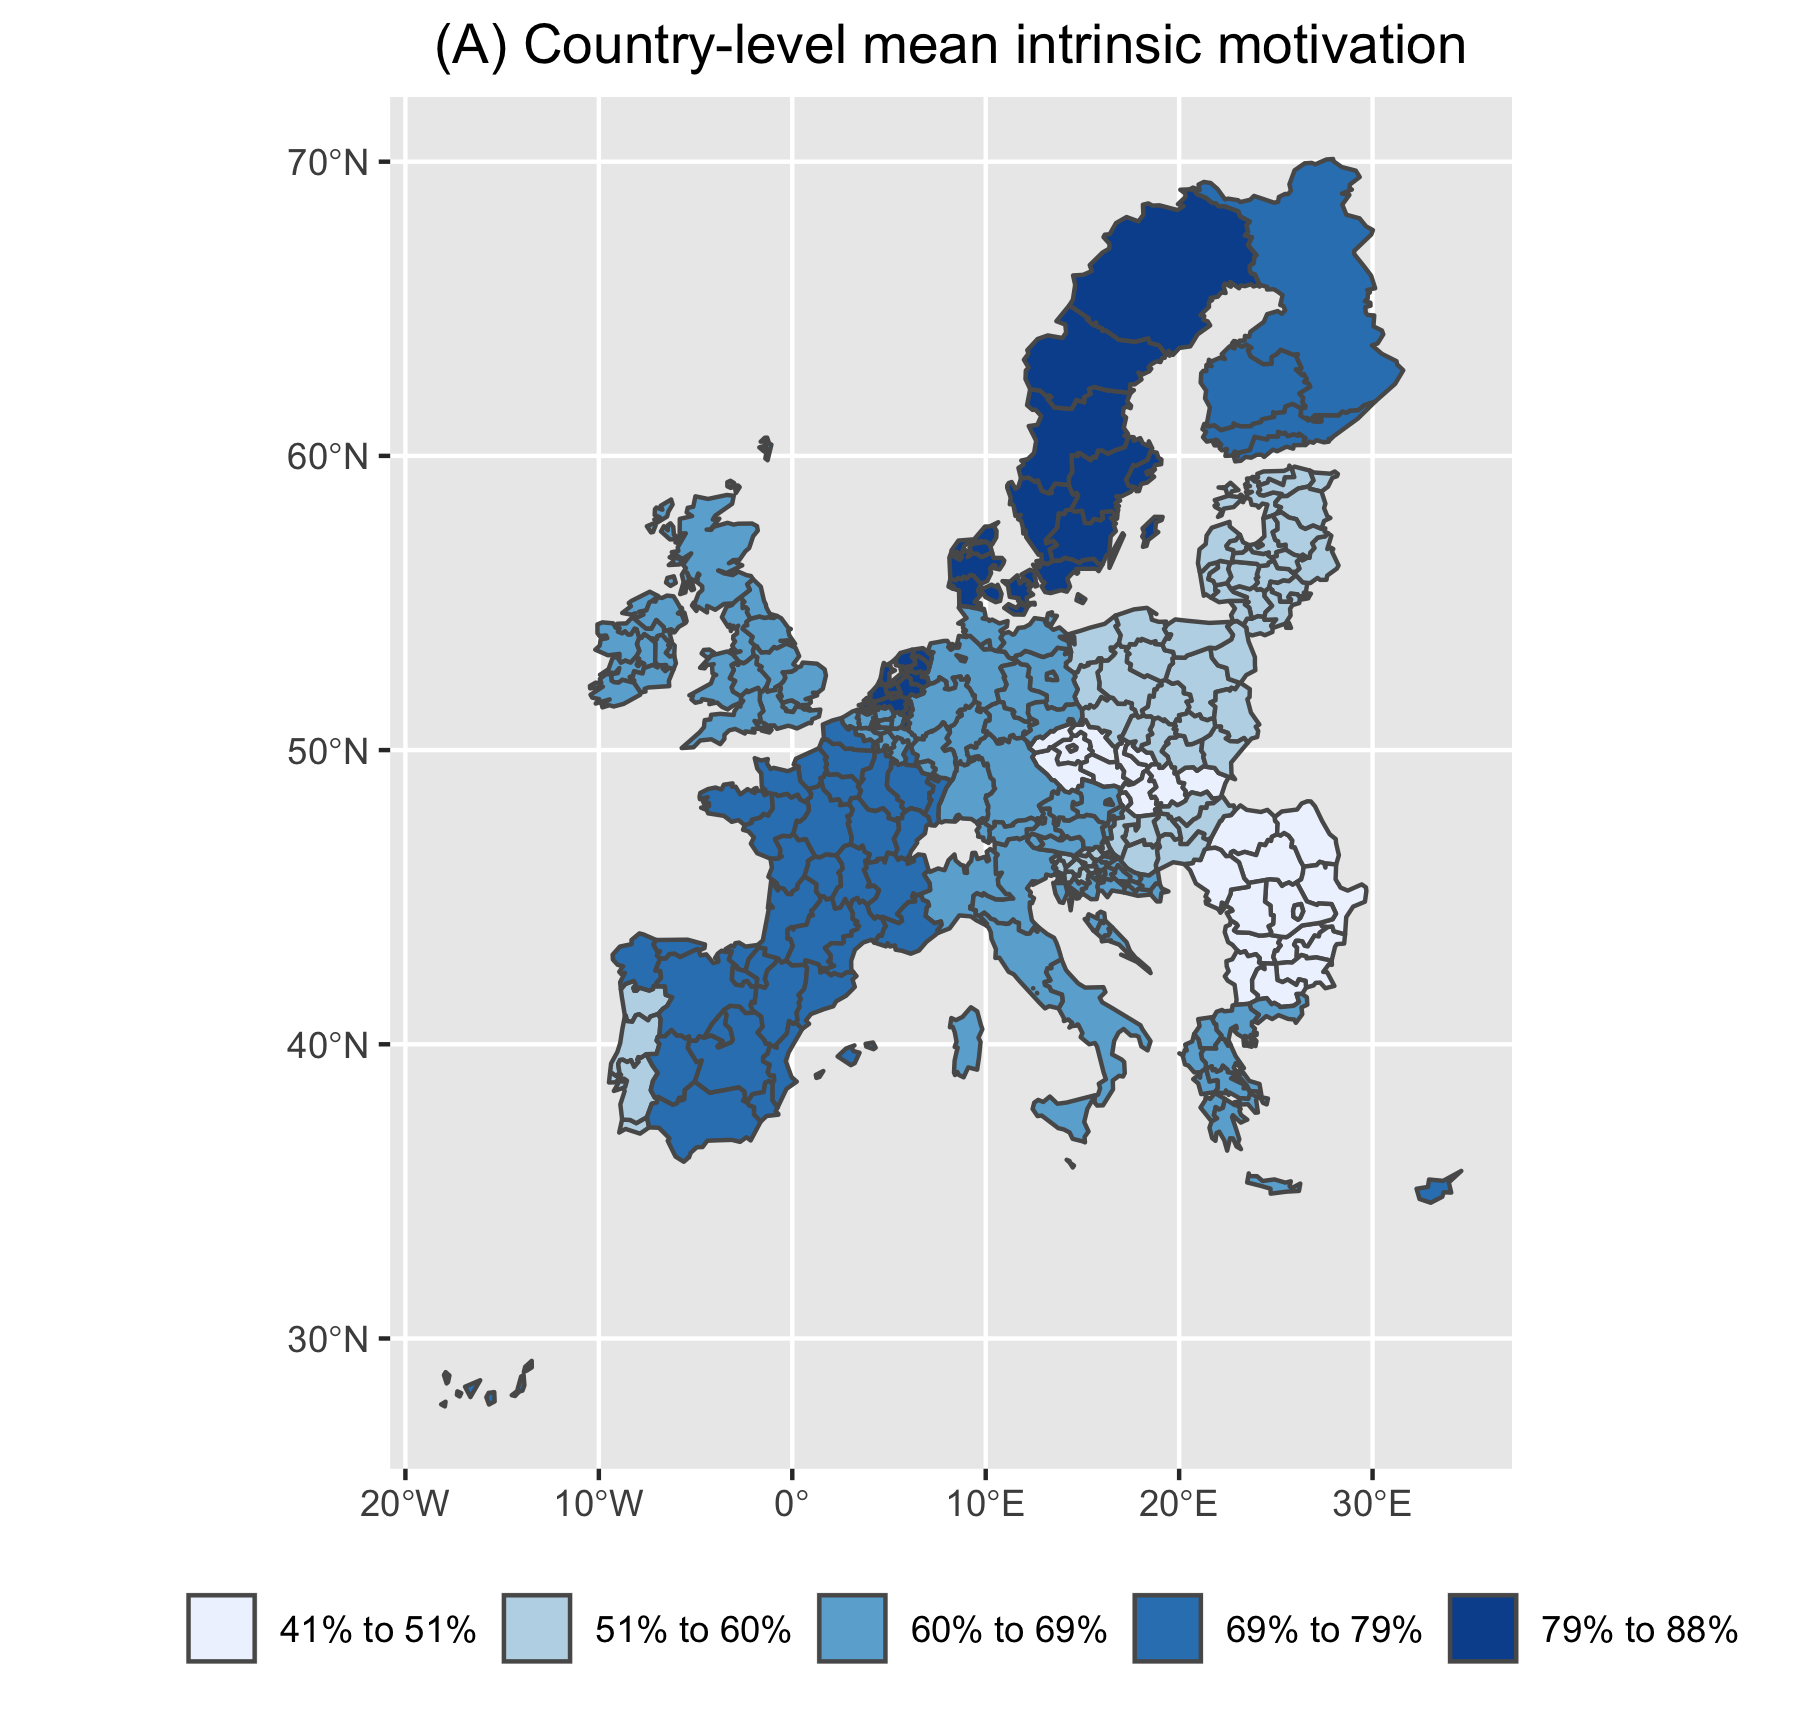
\includegraphics[width=\linewidth]{images/IM_countries.png}  
  %\caption{ }
\end{subfigure}
\begin{subfigure}{.48\textwidth}
  \centering
  % include second image
  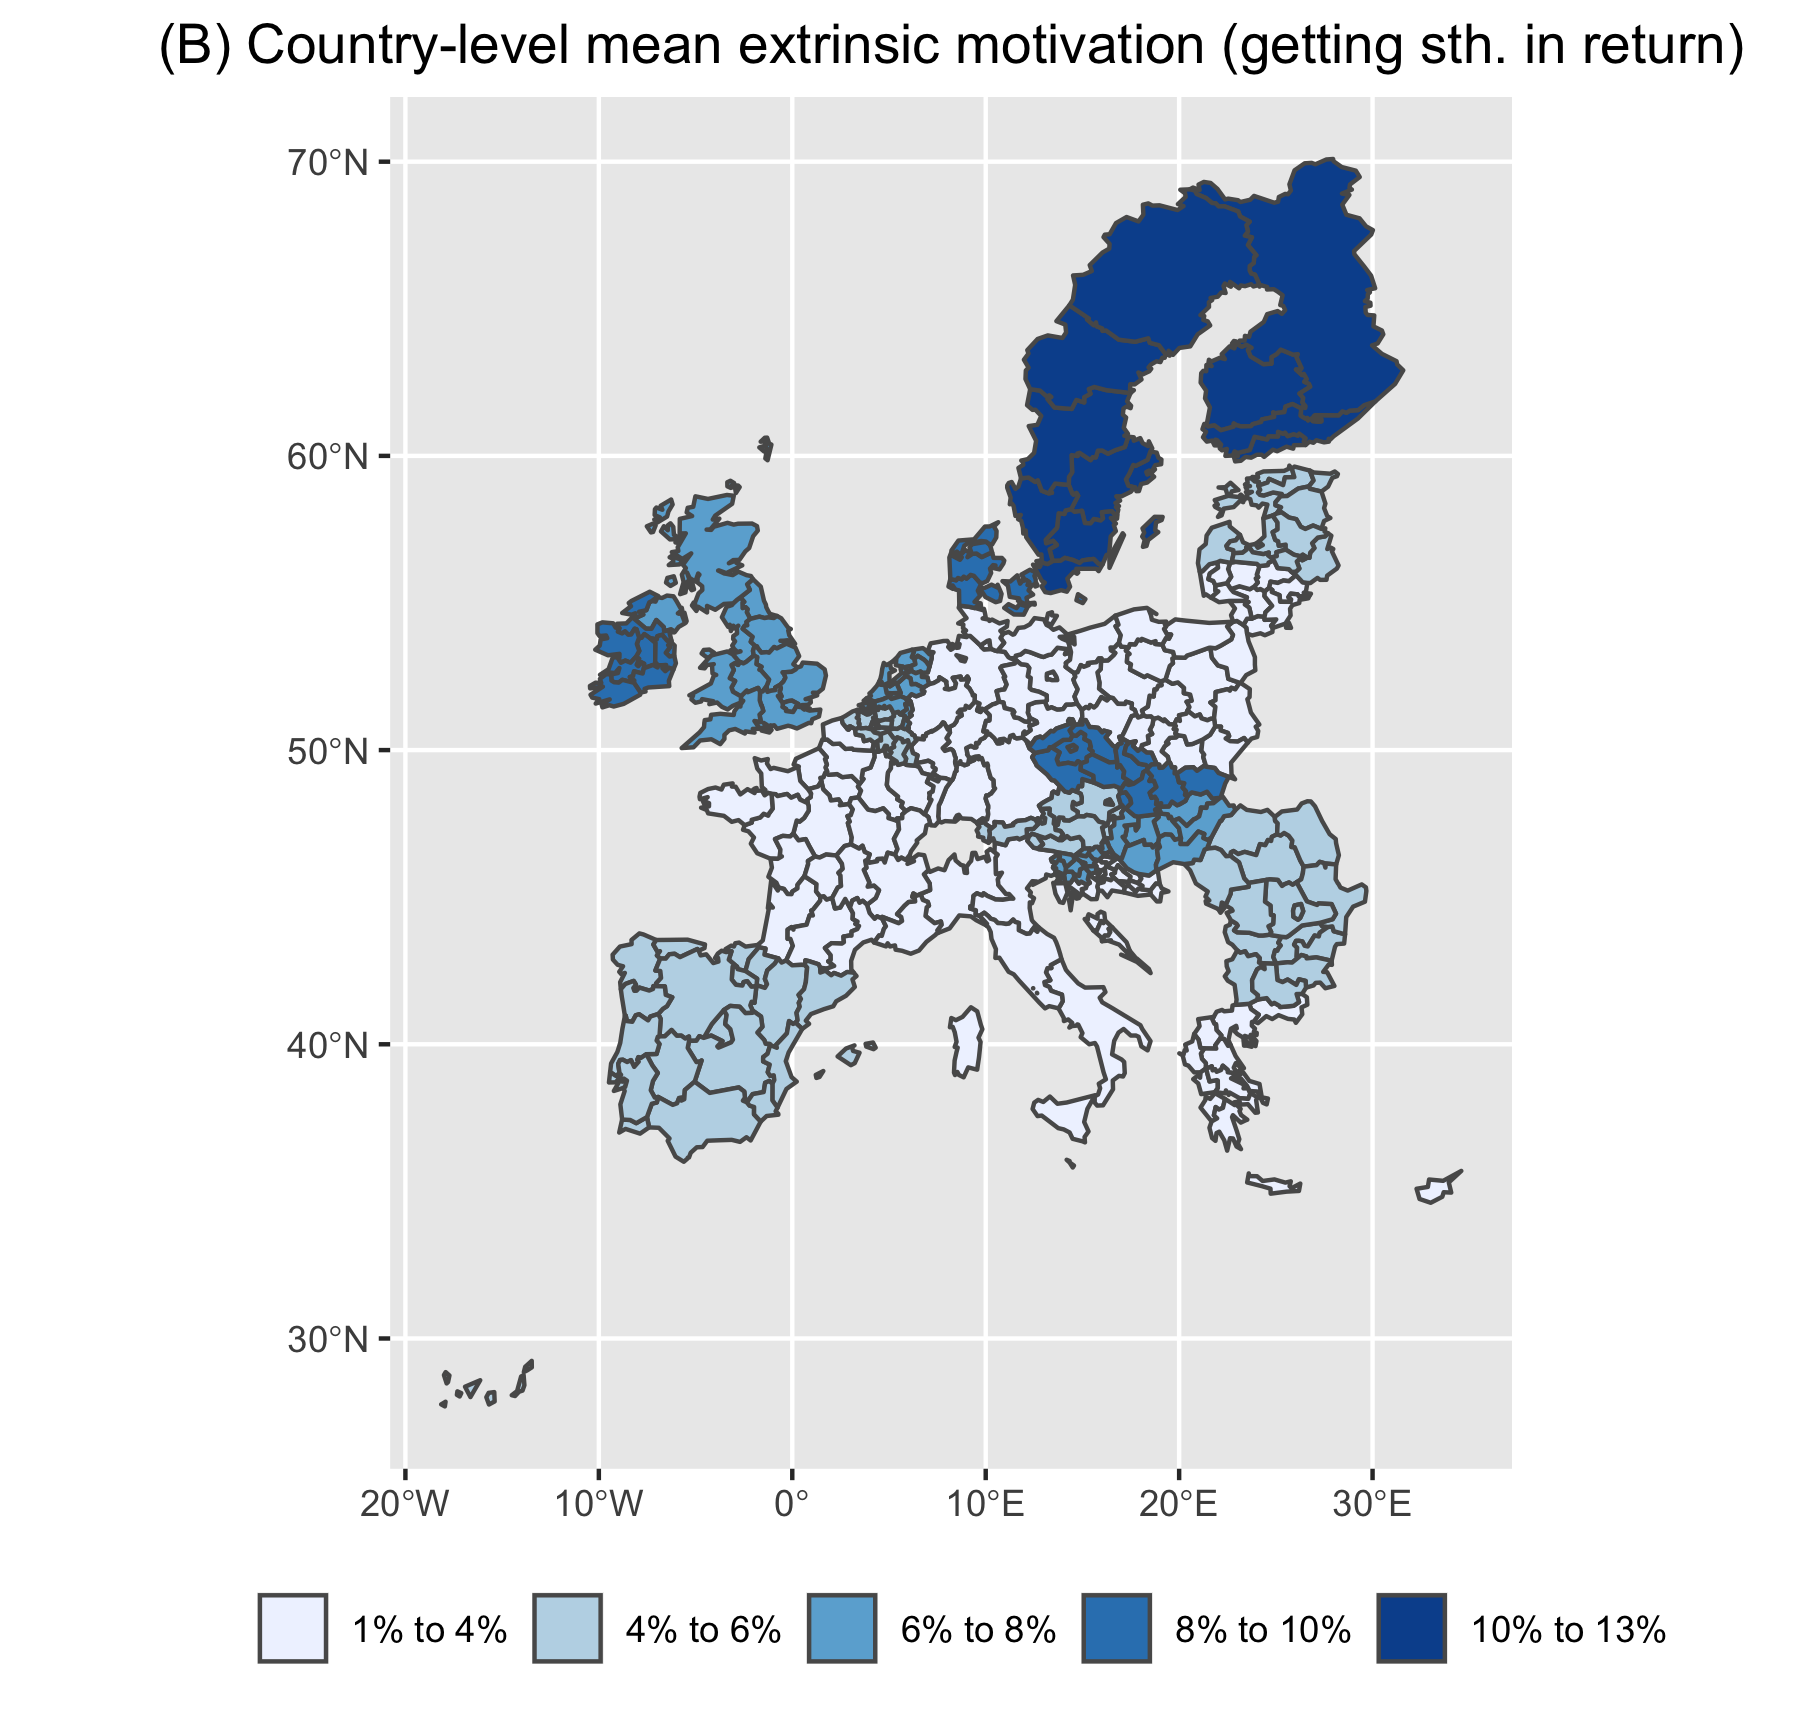
\includegraphics[width=\linewidth]{images/EM_get_return_countries.png}  
  %\caption{ }
\end{subfigure}

\newline

\begin{subfigure}{.48\textwidth}
  \centering
  % include third image
  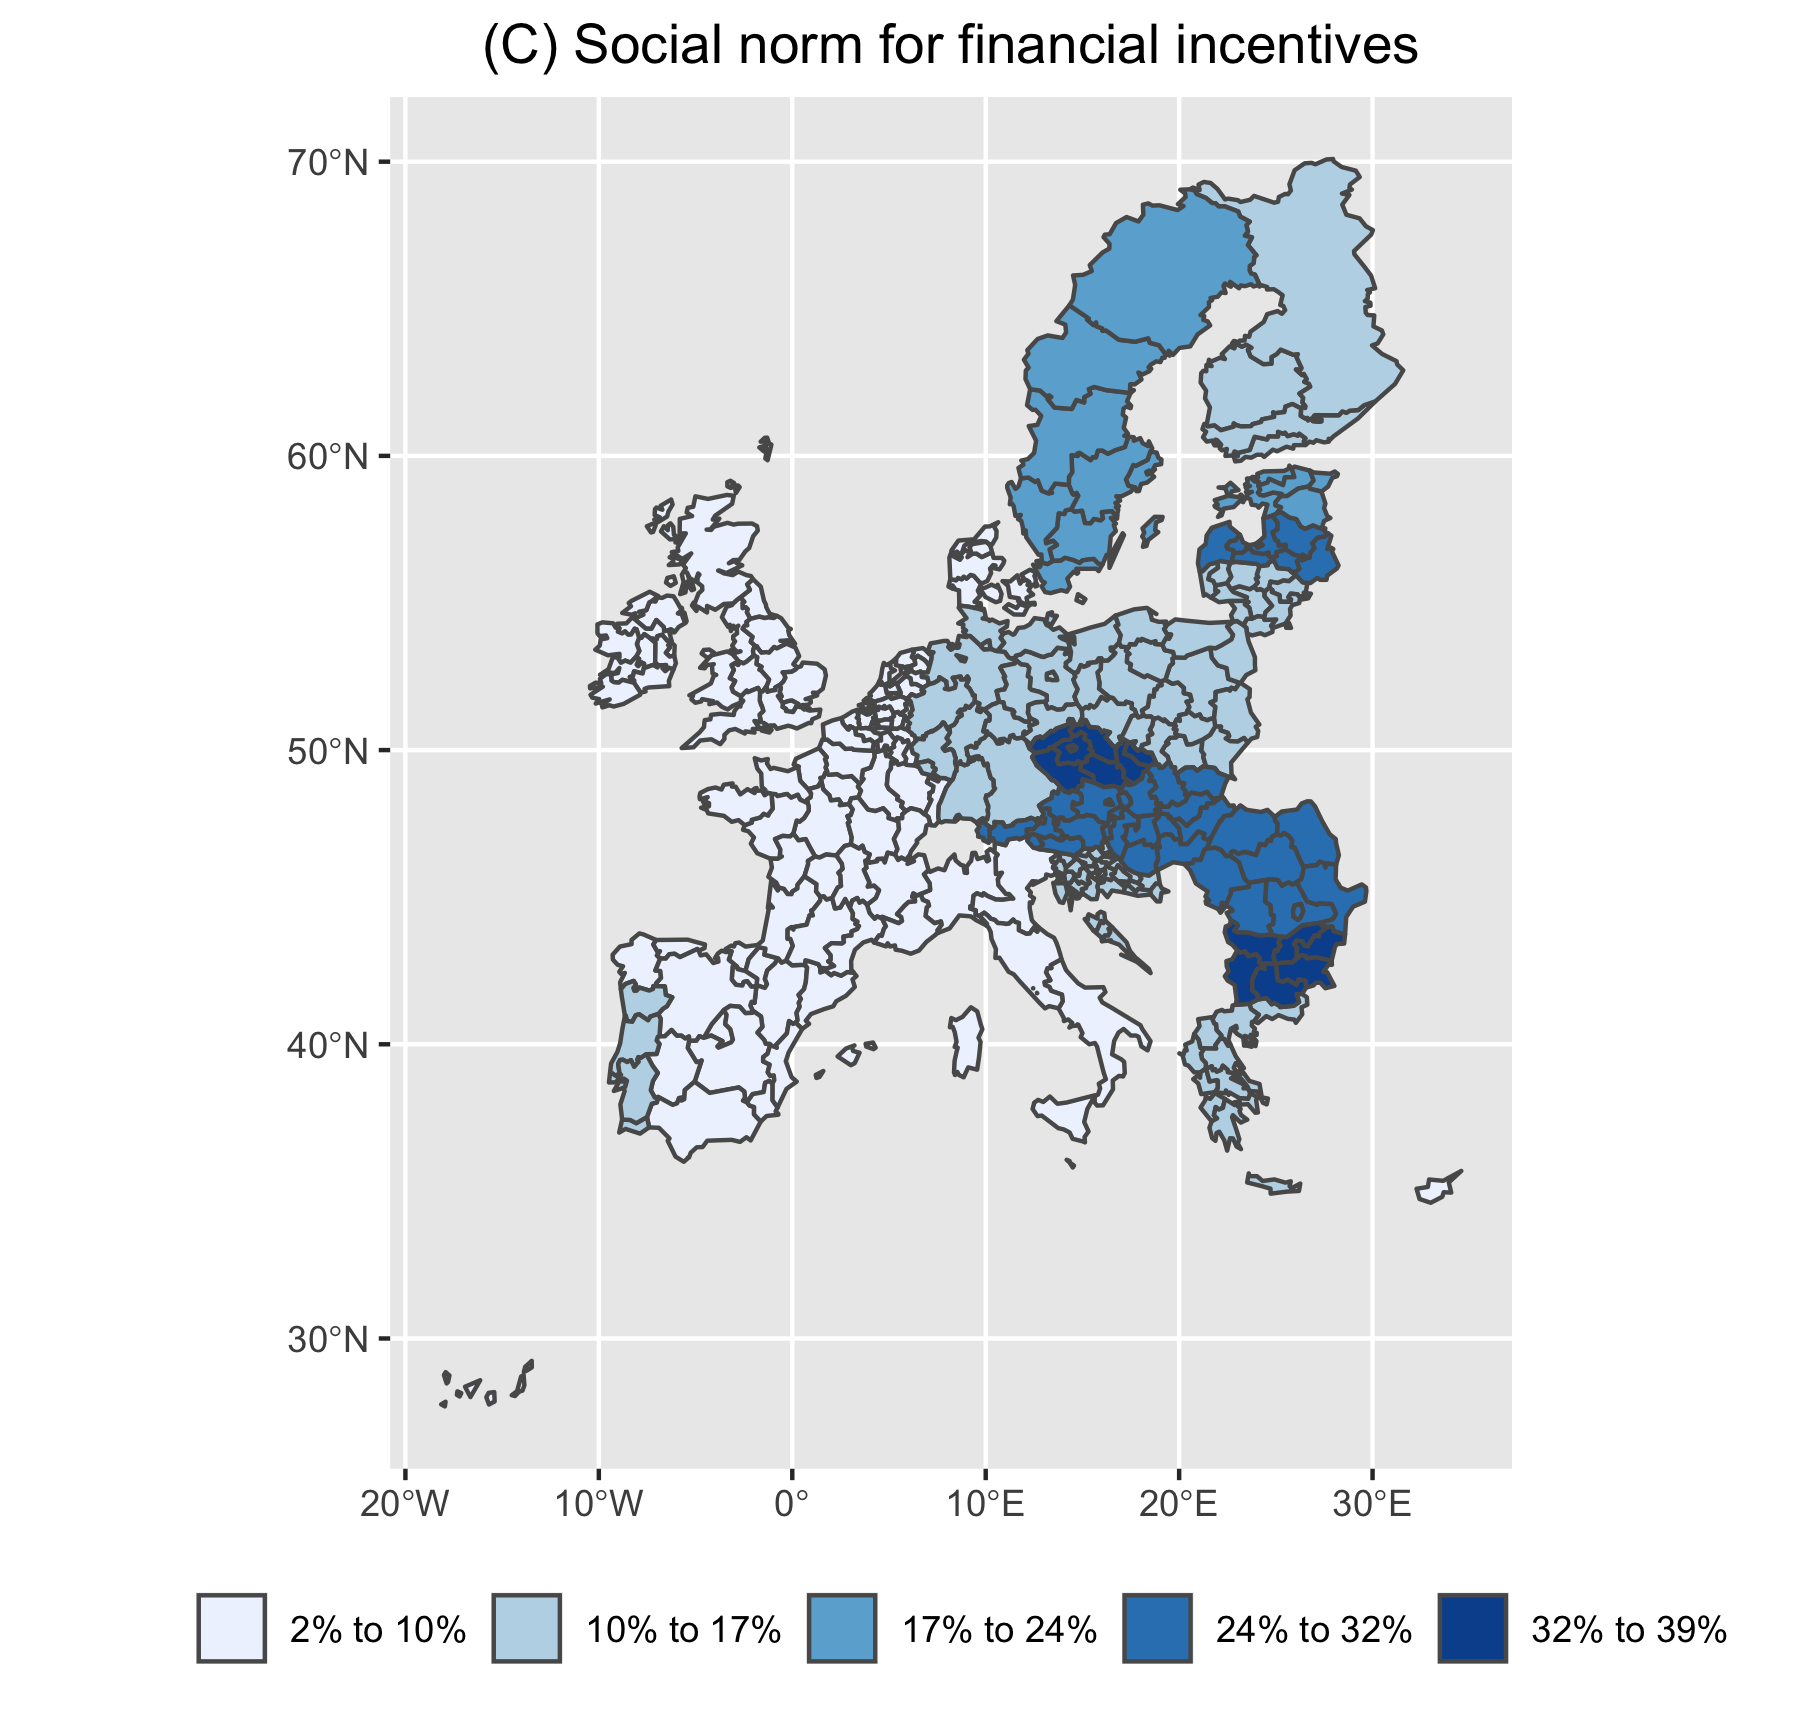
\includegraphics[width=\linewidth]{images/soc_financial_countries.png}  
  %\caption{ }
\end{subfigure}
\begin{subfigure}{.48\textwidth}
  \centering
  % include fourth image
  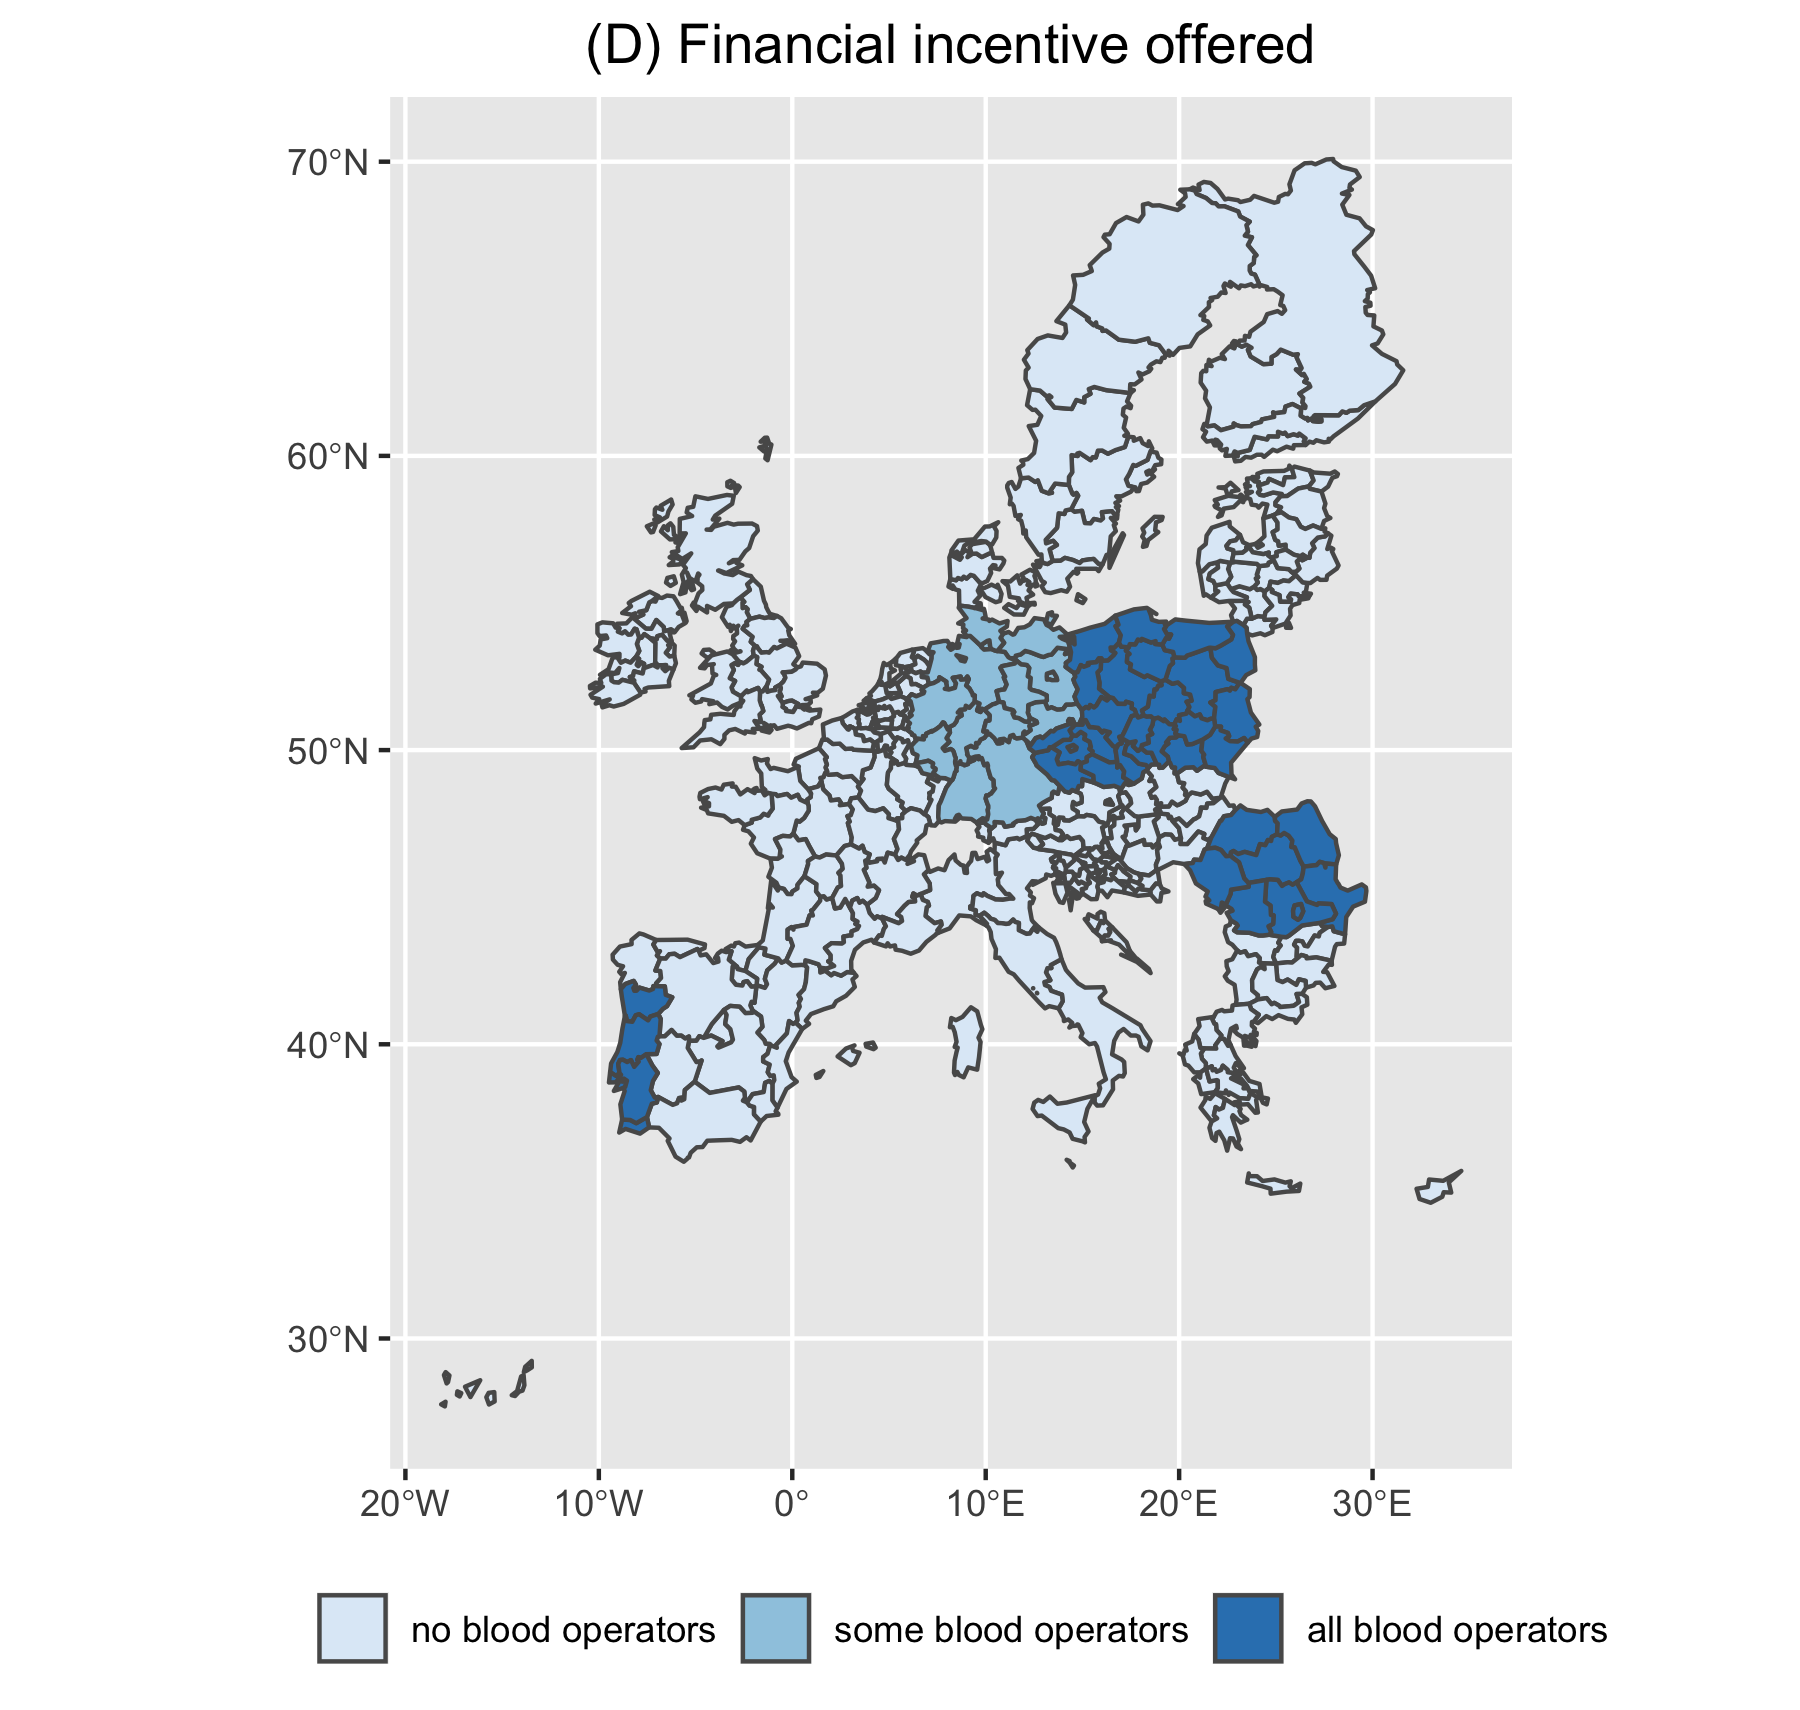
\includegraphics[width=\linewidth]{images/WB_incentive_countries.png}  
  %\caption{ }
\end{subfigure}
\caption{Country-level mean levels of (A) intrinsic motivation and (B) extrinsic motivation (in terms of mentioning “getting something in return” as a motivation to donate). (C) Aggregated country-level social norm regarding the acceptability of financial incentives for blood donation. (D) Financial incentives offered to blood donors in Europe.}
\label{fig:map_descr}
\end{figure}

\begin{table}[]
\begin{tabular}{l|l|l|l|l|l}
                 &                                              Variable  & Range                      & Mean                       & Std.         & n                          \\
Individual-level & Blood donation                                 & 0; 1                       & 0.38                       & -                          & 26532 \\
                 & Gender (female = 1)                            & 0; 1                       & 0.56  & -     & 26532 \\
                 & Age                                            & 18-99 & 51.29 & 17.81 & 26532 \\
                 & Education (No full-time education; ref.)       & -                          & 0.01  & -     & 25640 \\
                 & Education (≤15 years)                          & -                          & 0.17  & -     & 25640 \\
                 & Education (16-19 years)                        & -                          & 0.45  & -     & 25640 \\
                 & Education (≥20 years)                          & -                          & 0.37                       & -     & 25640 \\
                 & Cohabiting                                     & 0; 1                       & 0.65  & -     & 26476 \\
                 & Employed                                       & 0; 1                       & 0.49  & -                          & 26532 \\
                 & Difficulty paying bills: Never (ref.)          & -                          & 0.62  & -     & 26192 \\
                 & Difficulty paying bills: Sometimes             & -                          & 0.27  & -     & 26192 \\
                 & Difficulty paying bills: Most of the time      & -                          & 0.11                       & -     & 26192 \\
                 & Intrinsic motivation\footnote{Intrinsic motivation in the sample excluding respondents who did not donate in the past and are not willing to donate in the future had mean 0.8 (range: (0;1); n = 20961)}                          & 0; 1                       & 0.63  & -     & 26532 \\
                 & Extrinsic motivation (getting sth. in return)\footnote{Extrinsic motivation in the sample excluding respondents who did not donate in the past and are not willing to donate in the future had mean 0.07 (range: (0;1); n = 20961)
} & 0; 1                       & 0.06                       & -     & 26532 \\
                 & Number of children in household                & 0-15                       & 0.29  & 0.7   & 26527 \\
                 & Type of community: Large town (ref.)           & -                          & 0.27  & -     & 26518 \\
                 & Type of community: Mid-sized town              & -                          & 0.42  & -     & 26518 \\
                 & Type of community: Rural area                  & -                          & 0.31                       & -     & 26518 \\
Country-level    & Financial incentives: No blood operators       & -                          & 0.82                       & -                          & 28                         \\
                 & Financial incentives: Some blood operators     & -                          & 0.04                       & -                          & 28                         \\
                 & Financial incentives: All blood operators      & -                          & 0.14                       & -                          & 28                         \\
                 & Time incentives: No blood operator (ref.)      & -                          & 0.5                        & -                          & 28                         \\
                 & Time incentives: Dependent on employer         & -                          & 0.25                       & -                          & 28                         \\
                 & Time incentives: Independent of employer       & -                          & 0.25                       & -                          & 28                         \\
                 & Social norm (financial incentives)             & 0.02-0.39                  & 0.15                       & 0.1                        & 28                         \\
                 & Social norm (time incentives)                  & 0.12-0.70                  & 0.43                       & 0.15                       & 28                        
\end{tabular}
\caption{Descriptive statistics for the dependent variable and independent variables.}
\label{table:1}
\end{table}





\paragraph{Intrinsic motivation}

The full model (see supplementary Tables XX2 and XX3) with demographics and our effects of interest (including interactions between incentives and extrinsic motivation and social norms), as well as intercepts that are able to vary per country, revealed a significant contribution of intrinsic motivation ($b = 1.367, p < 0.0001$). That is, individuals who reported being motivated by the desire to help those in need, alleviate shortages, or support medical research were more likely to have donated blood. \footnote{As a robustness check, we implemented the same model on a subset of respondents, namely excluding those who were not given a chance to mention intrinsic motivational factors to donate (due to a lack of donation history and no reported willingness to donate in the future); for this sample we also found a significant positive effect of intrinsic motivation on blood donation (b = 0.095, p = 0.01).}

\paragraph{Extrinsic motivation, social norms and their interaction with financial incentives}

Testing the full model revealed a positive main effect of social norms regarding financial incentives ($b = 0.128, p < 0.05$), but a negative main effect of financial incentives themselves ($b = -0.512, p < 0.01$). This indicates that respondents in countries where incentives are offered are less likely to have donated blood in the past, but that individuals residing in countries with positive norms regarding financial incentives are more likely to have donated. The effect of extrinsic motivation (in terms of getting something in return as a motivation to donate) was positive but only marginally significant ($b = 0.108, p = 0.08$).\footnote{Similarly to the robustness check done with with intrinsic motivation, we also ran the former model on the subset of respondents which excluded those who had not previously donated and were not willing to donate; for this sample we did not find a significant positive association between extrinsic motivation (i.e. receiving something in return) and blood donation. In addition, the two other extrinsic motivation indicators related to respondents’ utility of monetary rewards (i.e., lack of employment and difficulty paying bills) had no positive effect on blood donation, contrary to our expectations. Instead, lack of employment was significantly associated with lower levels of blood donation and difficulty in paying bills was unrelated to donation behavior.}

Theoretically interesting are the interaction effects between incentives and extrinsic motivation on the one hand and incentives and social norms on the other. The former was marginally significant (for incentive = 1: $b = 0.283, p = 0.09$), such that respondents who indicated to be motivated by extrinsic motives tended to be more likely to have donated blood if they lived in a country where incentives are offered. \footnote{The predicted probabilities derived by the model of an “average” European woman (i.e., mean-aged, living with a partner and with secondary education) to donate blood is 39.6\% if she is extrinsically motivated and lives in a country offering incentives and 25.0\% if she is not extrinsically motivated living in a country offering incentives (on the other hand, her predicted probability to donate is 42.8\% when she is extrinsically motivated residing in a country without incentives opposed to 34.1\% when she is not extrinsically motivated residing in a country without incentives; see supplementary Fig. XXXA). Moreover, applying the robustness check to the model by employing the sample excluding respondents who had not previously donated and were not willing to donate found no significant interaction effect of extrinsic motivation and incentives (although it was in the expected direction; see also supplementary Fig. XXXC).}. The latter interaction effect between incentives and social norms was also in the expected direction, but not significant. Visual inspection of the predicted probabilities of blood donation for different levels of social norms and incentives (see Fig. \ref{fig:interactions}A) indicates that social norms are more positively associated with blood donation in countries where financial incentives are provided by all blood operators (blue line) than in countries where incentives are only provided by some blood operators (green line) or not at all (red line). That is, in countries where incentives are offered, an “average” European woman (i.e., mean-aged, living with a partner and with secondary education) has a predicted probability of donating blood of 20.4\% if the social norms regarding incentives are rather negative (as is the case in Portugal, where only 11.3\% of the population approves of financial incentives), but her predicted probability to donate increases to 31.0\% if the social norms are more positive (for instance in the Czech Republic, where 32.3\% of the population approves of financial incentives).

\begin{figure}[H]
\begin{subfigure}{\textwidth}
  \centering
  % include first image
  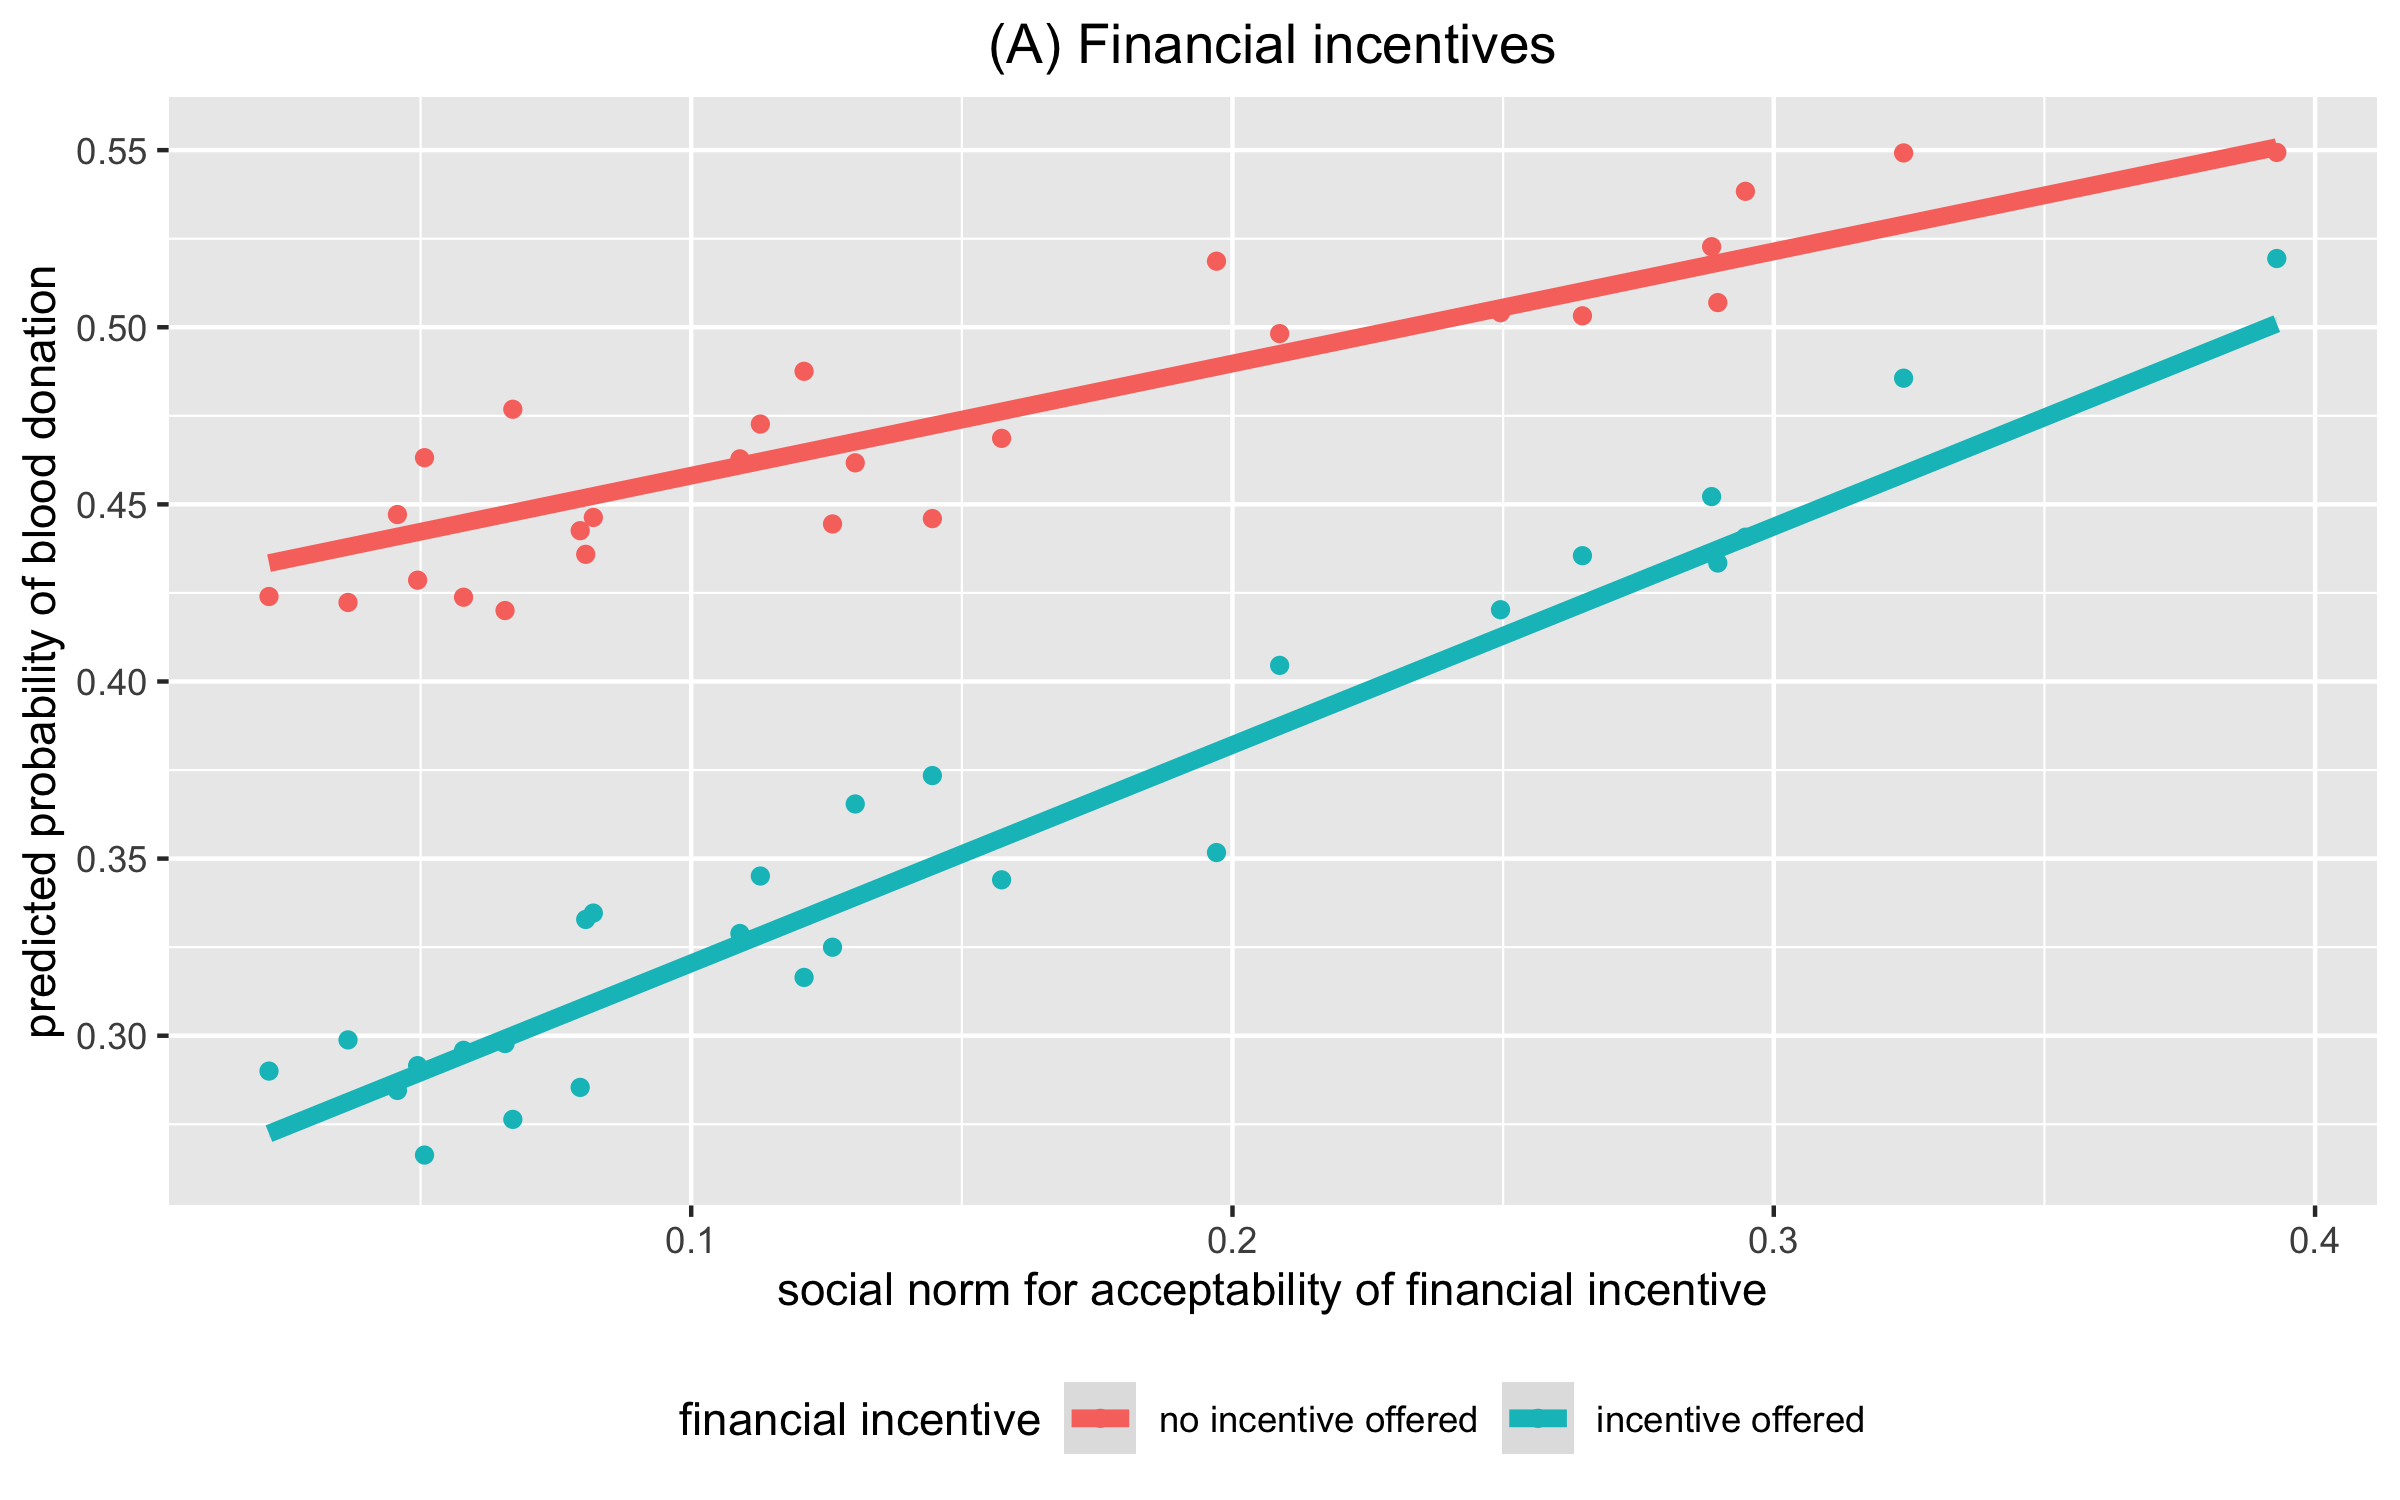
\includegraphics[width=.8\linewidth]{images/pred_SOC_incentives_financial_raw.png}  
  %\caption{Put your sub-caption here}
\end{subfigure}
\begin{subfigure}{\textwidth}
  \centering
  % include second image
  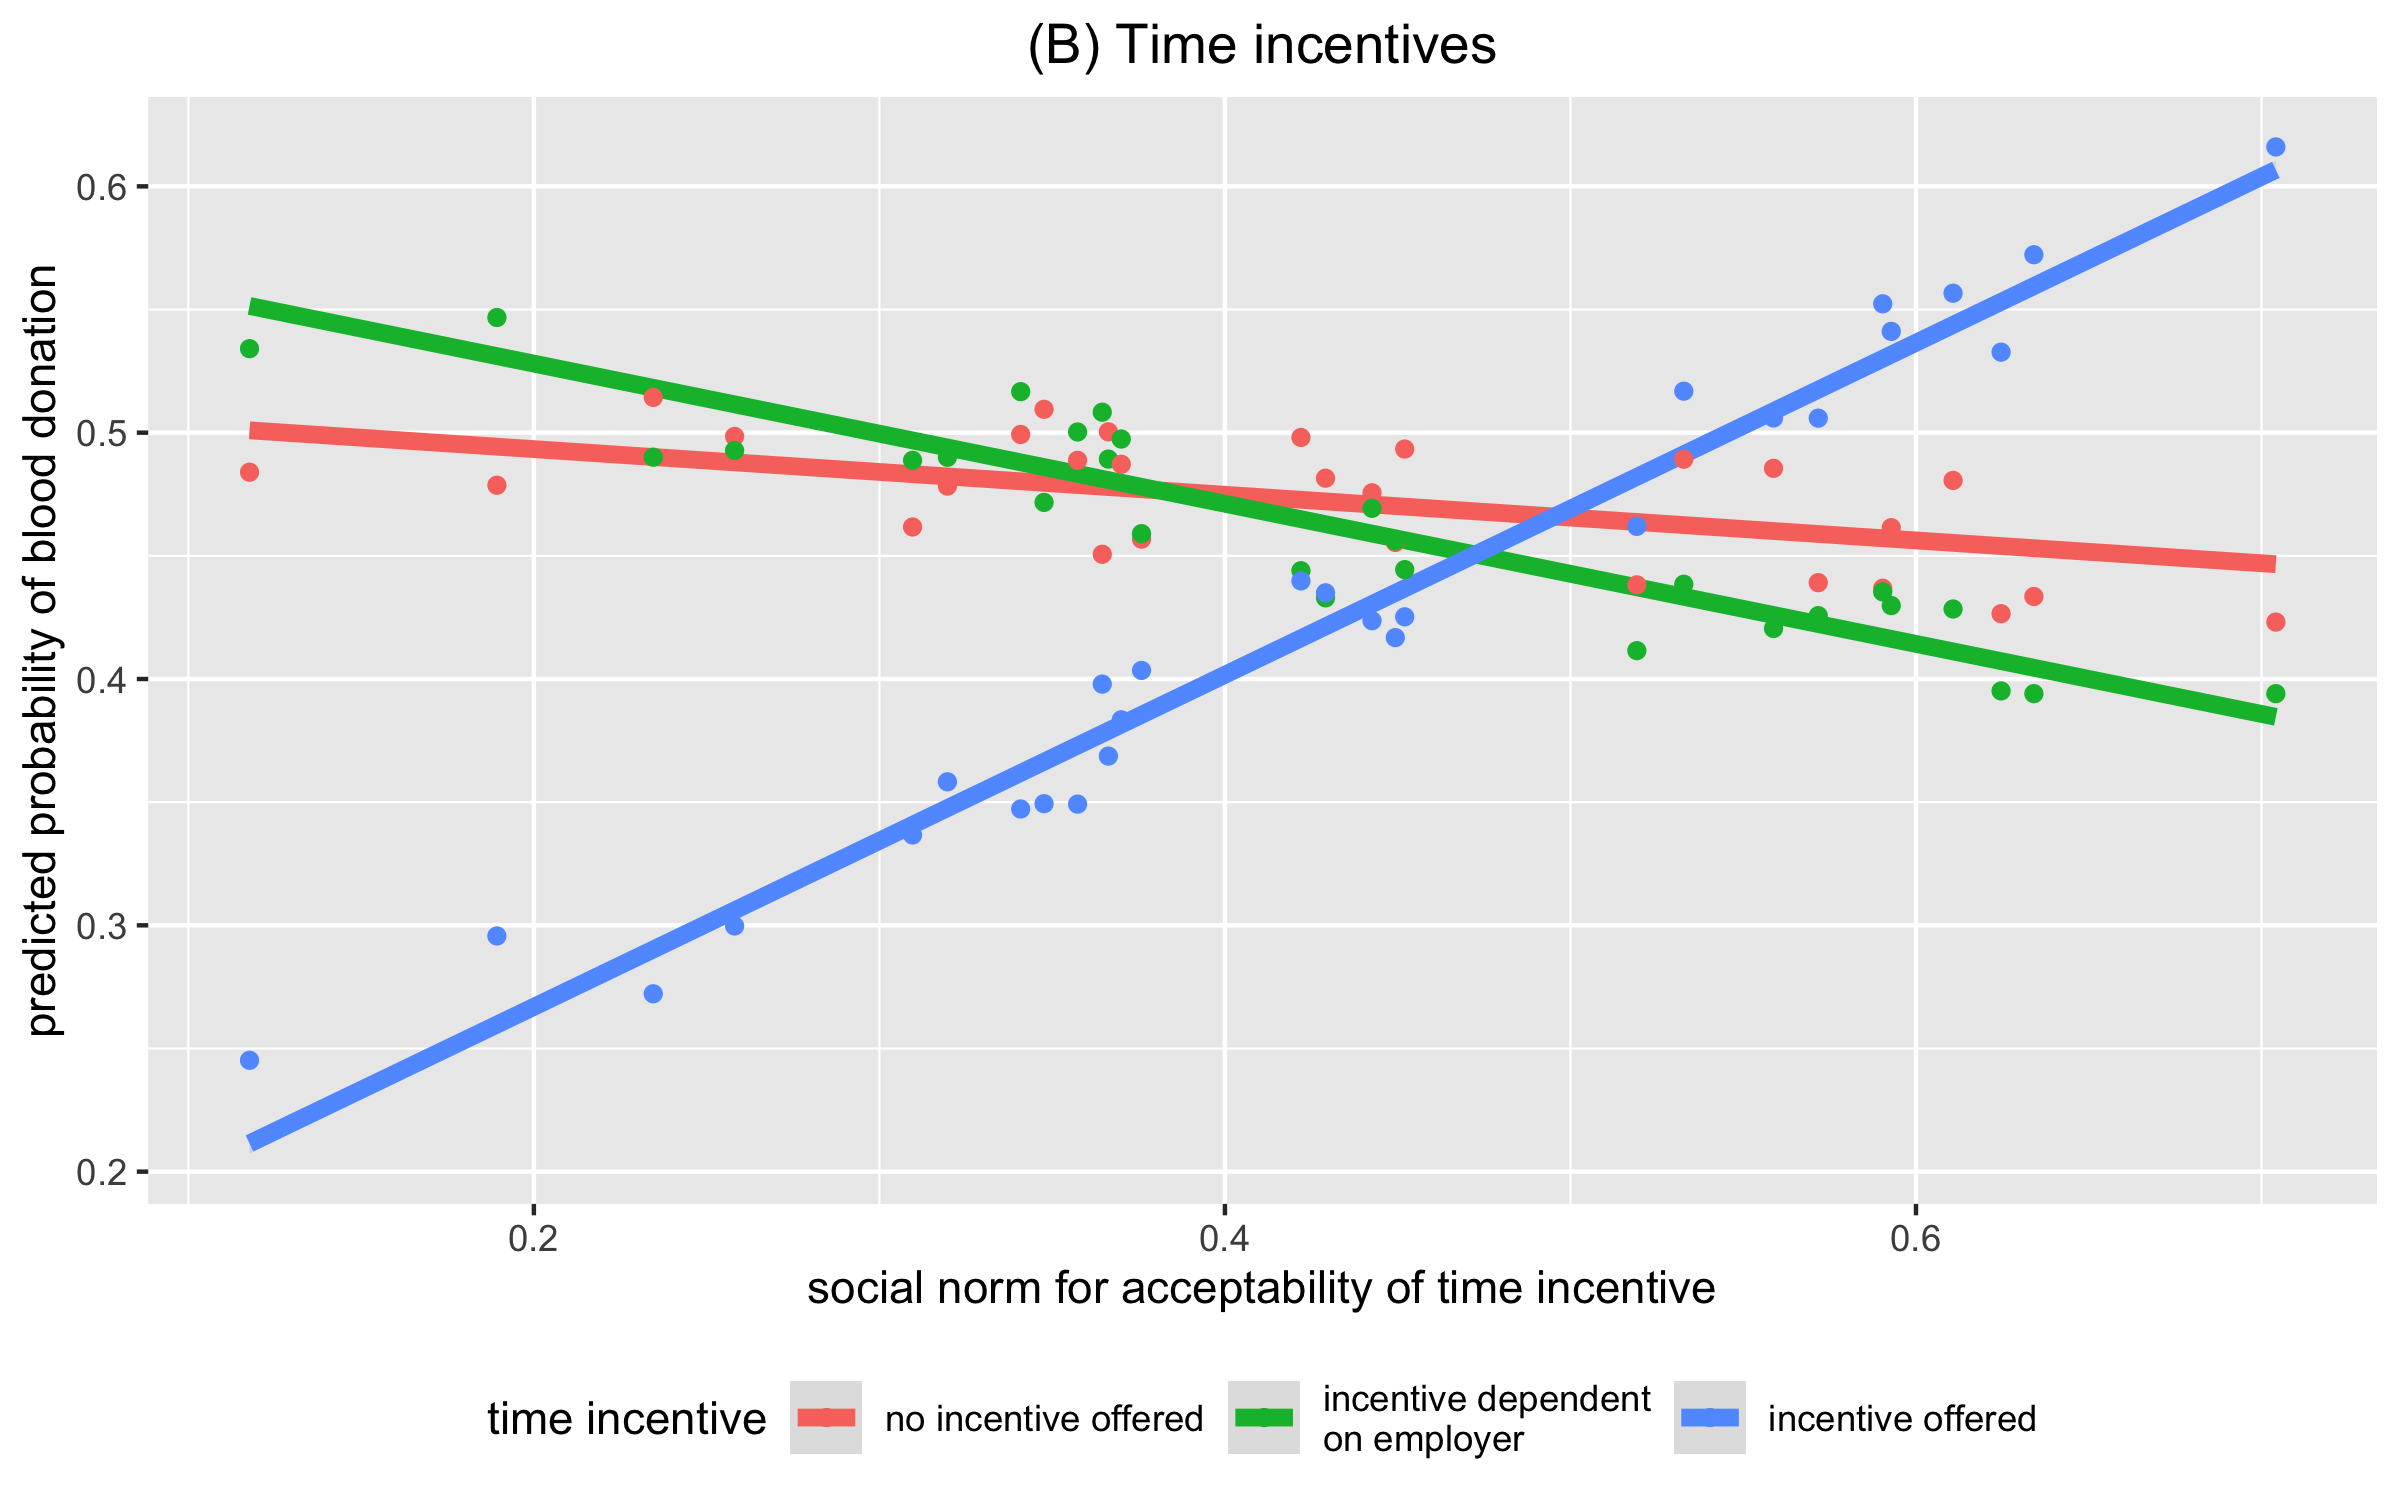
\includegraphics[width=.8\linewidth]{images/pred_SOC_incentives_time_raw.png}  
  %\caption{Put your sub-caption here}
\end{subfigure}
\caption{Scatter plot displaying predicted probabilities of donating blood for an “average” European woman (i.e., mean-aged, living with a partner and with secondary education) for varying values of (A) social norms regarding \textit{financial} incentives, grouped by different levels of financial incentives and (B) social norms regarding \textit{non-financial} incentives, grouped by different levels of non-financial incentives.}
\label{fig:interactions}
\end{figure}


\paragraph{Non-financial incentives}

In addition to providing information regarding which countries offer high-value \textit{financial} incentives, the expert survey furthermore showed that several countries employ high-value \textit{non-financial} incentives for blood donation, in particular time off work (see supp. Fig. YYYA, 14 out of 28 countries offer some kind of time incentive). Countries that offer time off work to blood donors (independent of employer policies) include Eastern European countries such as Bulgaria and Romania, but also Southern European countries such as Italy and Portugal. In other European countries, a subset of employers allow donors to take time off work for making the donation (for instance in Belgium, Croatia, Greece and Sweden). Country-level social norms regarding the acceptability of time incentives also varied substantially across countries (${X}^2(27) = 2436.6, p < 0.001$; values range from 11.8\% in Spain to 70.4\% in Sweden, see supp. Fig. YYYB). Social norms regarding time incentives were more positive (mean = 0.43) than those regarding financial incentives (mean = 0.15; Mann–Whitney $U(n_{1} = n_{2} = 28) = 736, p < 0.001$).

The associations between blood donation behavior and socio-demographics as well as intrinsic motivation were the same for the models additionally including time incentives as they were for financial incentives (see supp. Table XX4 and XX5). However, in contrast to the results pertaining to financial incentives, there was no main effect of non-financial incentives. That is, living in a country providing non-financial incentives had neither a positive or negative effect overall. In addition, there was neither a main effect for extrinsic motivation (in terms of getting something in return as a motivation to donate) nor for social norms regarding non-financial incentives. Instead, the model results revealed a significant positive interaction between non-financial incentives and social norms ($b = 0.527, p = 0.001$). This effect is depicted in Fig. \ref{fig:interactions}B: Individuals residing in countries offering time incentives had a 44.0\% predicted probability of donating if social norms were more positive (such as in Slovenia, where 63.4\% of the population approves of non-financial incentives), but only a 25.4\% predicted probability of donating if social norms were such that only 37.6\% of the population approves of non-financial incentives (as is the case in Italy). On the other hand, respondents living in countries not offering time incentives had a predicted probability to donate of 38.7\% when social norms were rather negative, and a predicted probability of 30.2\% when social norms were more positive.

In addition, we found a positive trend in the interaction between non-financial incentives and extrinsic motivation ($b = 0.256, p = 0.09$). That is, individuals tended to have a higher probability of donating blood if they lived in a country with time incentives and were extrinsically motivated than those residing in countries providing time incentives but not being extrinsically motivated (see supp. Fig. YYYB).

\section{Discussion}

\textbf{Author contributions}: E-MM and CG conceived the project idea. All authors contributed to the design and analysis plan. CG implemented the theoretical model, conducted the expert survey, performed statistical analyses, and wrote the first draft of the manuscript. All authors discussed the results and contributed to the final paper.

\textbf{Acknowledgements}: This work was supported by the European Research Council (ERC) under grant agreement 802227. The work by PW at the Lilly Family School of Philanthropy is funded through a generous donation by the Stead Family, her work at the Vrije Universiteit Amsterdam is funded by the Dutch Charity Lotteries.

\textbf{Conflict of interest}: The authors have disclosed no conflict of interest.

%Sample figure:
%
%\begin{figure}
%Figure here.
%
%\caption{Caption for figure below.}
%\begin{figurenotes}
%Figure notes without optional leadin.
%\end{figurenotes}
%\begin{figurenotes}[Source]
%Figure notes with optional leadin (Source, in this case).
%\end{figurenotes}
%\end{figure}
%
%Sample table:
%
%\begin{table}
%\caption{Caption for table above.}
%
%\begin{tabular}{lll}
%& Heading 1 & Heading 2 \\ 
%Row 1 & 1 & 2 \\ 
%Row 2 & 3 & 4%
%\end{tabular}
%\begin{tablenotes}
%Table notes environment without optional leadin.
%\end{tablenotes}
%\begin{tablenotes}[Source]
%Table notes environment with optional leadin (Source, in this case).
%\end{tablenotes}
%\end{table}

\bibliographystyle{aea}
\bibliography{bib_P1.bib}

% The appendix command is issued once, prior to all appendices, if any.
\appendix

\section{Mathematical Appendix}

\end{document}

